%!TeX program = pdflatex
\documentclass{scrbook}

% ---------------------------
% Konfiguration & eigene Kommandos
% ---------------------------
\usepackage{setspace}
\KOMAoptions{ twoside=true, open=any, headings=optiontoheadandtoc,parskip=true,fontsize=8.5pt,parskip=half-}
\usepackage{geometry}
\geometry{
	paperwidth=154mm,
	paperheight=216mm,
	layout=a5paper,
	lmargin=1cm,
	tmargin=1.5cm,
	textheight=173mm,
	textwidth=128mm,
	includefoot,
	footskip=30pt,
	layoutoffset=3mm
}




%%%%%% Print %%%%%%%%%%%%%%%%%%%%%%%%%%%%%%%%%%%%%%%%%%%%%%%%%%%%%%%%

% Lege die ICC-Datei PSOcoated_v3.icc ins Projektverzeichnis
%\usepackage[x-4]{pdfx} % erzeugt PDF/X-4 mit OutputIntent
% pdfx nimmt standardmäßig die im Projekt liegende ICC als OutputIntent, z. B. PSOcoated_v3.icc

%%%%%% Portraits %%%%%%%%%%%%%%%%%%%%%%%%%%%%%%%%%%%%%%%%%%%%%%%%%%%%

\usepackage{float}
\usepackage{wrapstuff}
\usepackage{wrapfig}


%%%%%% Section titles %%%%%%%%%%%%%%%%%%%%%%%%%%%%%%%%%%%%%%%%%%%%%%%

\setcounter{secnumdepth}{0}
\setcounter{tocdepth}{2}

\RedeclareSectionCommand[
	afterskip = {0.4ex plus 0.2ex},
	beforeskip = {-1ex plus -1ex minus -.2ex},
	font={\LARGE},
]{section}

\RedeclareSectionCommand[
	afterskip = {.4ex plus .2ex},
	beforeskip = {-0.25ex plus -1ex minus -.2ex},
	font={\Large},
]{subsection}
	
\DeclareNewSectionCommand[
	afterskip = {.4ex plus .2ex},
	beforeskip = {-0.25ex plus -1ex minus -.2ex},
	indent=0pt,
	font={\LARGE},
	style=section,
	level=1,
	tocindent=0pt,
	toclevel=1,
	tocnumwidth=2em,
	tocstyle=chapter,
]{sectionPart}

\RedeclareSectionCommand[
afterskip = {-1em},
beforeskip = {0ex plus -1ex minus .2ex},
runin=false,
]{paragraph}

\setparsizes{0pt}%infdent
{9pt}%vskip
{0pt plus 1fil}


%%%%%% Section headings %%%%%%%%%%%%%%%%%%%%%%%%%%%%%%%%%%%%%%%%%%%%

\usepackage{ifthen}
\newcounter{secautolabel}
\AddtoDoHook{heading/endgroup}{\setautolabel}
\newcommand*{\setautolabel}[1]{%
  	\stepcounter{secautolabel}%
  	\label{sec:autolabel:\thesecautolabel}%
	\def\sname{#1}
	\ifthenelse{\equal{#1}{sectionPart}}{
		\def\sname{section}
	}{}
  	\expandafter\xdef\csname \sname title\endcsname{%
    	\noexpand\nameref{sec:autolabel:\thesecautolabel}%
  	}%
}


%%%%%% Font, Encoding etc. %%%%%%%%%%%%%%%%%%%%%%%%%%%%%%%%%%%%%%%%%%

\usepackage[utf8]{inputenc}
\usepackage[T1]{fontenc}
\usepackage[ngerman]{babel}
\usepackage{amsmath,amsfonts,amssymb}
\usepackage[default,light,lf]{FiraSans}
\usepackage{pifont}


%%%%%% Colors %%%%%%%%%%%%%%%%%%%%%%%%%%%%%%%%%%%%%%%%%%%%%%%%%%%%%%%

\usepackage{xcolor,colortbl}

\definecolor{fscolor}{RGB}{11,161,226}
\definecolor{petrol}{HTML}{216477}
\definecolor{lecegreen}{HTML}{0aa3e4}


%%%%%% tikz %%%%%%%%%%%%%%%%%%%%%%%%%%%%%%%%%%%%%%%%%%%%%%%%%%%%%%%%%

\usepackage{tikz}
\usetikzlibrary{calc}
\usetikzlibrary{shapes.geometric}
\usetikzlibrary{decorations}


%%%%%% Tabellen %%%%%%%%%%%%%%%%%%%%%%%%%%%%%%%%%%%%%%%%%%%%%%%%%%%%%

\usepackage{tabularx}
\usepackage{makecell}
\usepackage{tabularray}
\usepackage{multicol}
%\usepackage{tocbasic}        % Inhaltsverzeichnis verändern schiebt es nach unten oder oben

%%%%%% Sonstiges %%%%%%%%%%%%%%%%%%%%%%%%%%%%%%%%%%%%%%%%%%%%%%%%%%%%

\usepackage{qrcode}

\usepackage[]{graphicx}

\usepackage[export]{adjustbox}% http://ctan.org/pkg/adjustbox

\usepackage{caption}

\usepackage{array}
\usepackage{forarray}
\usepackage{forloop}

\usepackage{enumitem}
\usepackage{etoolbox}
\usepackage[german=quotes]{csquotes}
\usepackage{scrlayer-fancyhdr}

\usepackage{microtype}
\usepackage{lipsum}           % Platzhaltertext
\usepackage{pdfpages}         % Für PDF-Einbindung

% Flattersatz & Trennung aus
\usepackage{ragged2e}
\AtBeginDocument{\RaggedRight}      % global linksbündig (kein Blocksatz)
\usepackage[none]{hyphenat}         % Silbentrennung aus
\emergencystretch=1em               % etwas Puffer gegen overfull lines
\setlength{\RaggedRightParindent}{0pt}

% URLs besser umbrechen (Option muss vor hyperref rein)
\PassOptionsToPackage{hyphens}{url}

\usepackage[
	linktoc=black,
	linkcolor=.,
	urlcolor=fscolor,
	breaklinks=true,
	colorlinks,
	bookmarks,
	plainpages=false,
	citecolor=gray,
]{hyperref}
\urlstyle{same}


% URL-Umbrüche noch flexibler
\Urlmuskip=0mu plus 2mu


% Checkliste
\newlist{todolist}{itemize}{2}
\setlist[todolist]{label=$\square$}


\newcounter{pagehead}
\input{1.0.0.0_config/footer_header.tex}
\input{1.0.0.0_config/commands.tex}


\raggedbottom

% ---------------------------
% Dokumentbeginn
\begin{document}
% ---------------------------


% ---------------------------
% Backcover
\includepdf{./7.0.0.0_umschlag/Cover.pdf}
% ---------------------------

\newpage
\thispagestyle{empty}
\null
\newpage


\pagenumbering{gobble}
%Vorwort 
\section*{\textbf{How to Ersti-Heft}}

\textbf{Moin und willkommen im Studium!}\\
%Die Absicht und die Idee hinter dem Heft 
Dieses Heft ist die erste Ausgabe meines Ersti-Hefts für alle Informatik-Erstis an der H-BRS.
Der Studienstart ist eine spannende Zeit – voller neuer Eindrücke, Menschen und tonnenweise Informationen. Da verliert man schnell mal den Überblick.

\vspace{-2mm}

Genau dabei soll dir dieses Heft helfen: Es gibt dir Orientierung und erleichtert dir den Einstieg ins Studium.

\vspace{-2mm}

%Dieses Heft ist nicht nur auf Papier gedacht, sondern 
Dieses Helft funktioniert am besten in Kombination mit der dazugehörigen PDF.  
Ganz ohne mühsames abtippen: Die wichtigsten Inhalte findest du direkt als \textbf{QR-Code zum Einscannen} oder als \textbf{Link} im Heft und in der PDF, um auf die jeweiligen Ressourcen zuzugreifen. Lass dich nicht von den vielen Seiten abschrecken. \\
%Das Heft ist so aufgebaut, dass du die Kapitel lesen kannst, die dich interessieren. Du musst nicht alles von vorne bis hinten durchlesen.

\underline{\textbf{Bitte beachte:}} Manche Informationen können sich nach Redaktionsschluss ändern. Dies ist leider nicht zu verhindern. In der PDF dieses Heftes und über die verlinkten Seiten stehen dir jedoch immer die \textbf{’’aktuellsten Ressourcen’’} zur Verfügung. Basierend darauf wie oft die Webseiten aktualisiert werden, kann es sein, dass du dort neuere Informationen findest als zum aktuellen Stand in diesem Heft/PDF.\\
Falls du dir nicht sicher bist, ob eine Information noch aktuell ist, schau am besten auf die verlinkte Seite oder kontaktiere die dort angegebenen Ansprechpartner.\\
Frag lieber einmal zu viel nach, als einmal zu wenig!

%Das sich der Druck verzögert erhaltst du diese PDF zur gleichen Zeit wo du das Heft erhalten hättest sollen. Ich liefere es dir nach -Timo

%\vspace{-1mm}

\textbf{Tipp 1:} Speichere die PDF auf deinem Handy oder Tablet ab, damit du sie immer griffbereit hast.
\textbf{Tipp 2:} Benutze das Inhaltsverzeichnis um schnell wo hinzukommen. Du kannst so über die PDF auch direkt zu den Kapiteln springen.\\
\textbf{Tipp 3:} \texttt{STRG+F} ist dein Freund wenn du noch effizenter sein willst beim Suchen (Falls du es nicht kennst, der Shortcut hilft um in Objekten nach Begriffen zu suchen).

\vspace{-2mm}

\medskip
\noindent
\textbf{Sicherheit der QR-Codes}  
Alle QR-Codes in diesem Heft werden automatisch im LaTeX erzeugt. Jeder Code verweist ausschließlich auf den Link, der direkt darunter, daneben oder darüber steht. So gibt es keine Verwechslungen und kein Risiko durch manipulierte QR-Codes.

Viel Erfolg und einen guten Start ins Studium wünscht dir\\
\textbf{Timo Mansfeld}

\vspace{-5mm}

\begin{center}
  %\vspace{-5mm}
  % Beispiel QR-Code mit Link zum PDf vom Heft
  \vfill
  \small \textbf{Hier bekommst du die PDF des Hefts.}\\
  \small\href{https://drive.google.com/drive/folders/1Pqqn5CicX540Pdtz4d6UKSQVwXJDEsOY?usp=sharing}{Google Drive Ersti-Heft}\\
  \vspace{1mm}
  \qrcode[height=45mm]{https://drive.google.com/drive/folders/1Pqqn5CicX540Pdtz4d6UKSQVwXJDEsOY?usp=sharing}\\
  \vfill
\end{center}




% Inhaltsverzeichnis
\clearpage
\begingroup
    % Kapitelkopf-Abstand (nur in dieser Gruppe) deutlich verkleinern
    \RedeclareSectionCommand[beforeskip=-0cm]{chapter} % ≈ 2 cm höher
    \tableofcontents
\endgroup


% ---------------------------
% Dekan und Fachschaft
% ---------------------------


\PART{Begrüßung}
    \pagenumbering{arabic}  % => arabisch
    \setcounter{page}{1}    % optional, hier korrekt
	\newpage
\begin{wrapstuff}[type=figure, r, width=0.6\textwidth, top=1]
    \setlength{\abovecaptionskip}{8pt plus 3pt minus 2pt}
    \centering
    \includegraphics[width=\textwidth]{./2.0.0.0_content/photos/dekanat.png}
    \\[0.5em]
    {\small Das Dekanat, }
    {\small v.l.n.r.: Prof.\ Dr.\ Sascha Alda (Dekan), Prof.\ Dr.\ Matthias Bertram (Prodekan)}
\end{wrapstuff}

\section{Dekanat des Fachbereichs Informatik}

Liebe Erstsemester,

herzlich willkommen am Fachbereich Informatik! Mit Ihrem Studienbeginn schlagen Sie ein neues Kapitel in Ihrem Leben auf – in einem Fachgebiet, das unsere moderne Welt wie kaum ein anderes prägt. Informatik bedeutet weit mehr als Programmieren. Sie ist die Basis für aktuelle Entwicklungen in der Künstlichen Intelligenz, Cyber Security, Wirtschaftsinformatik, Spiele-Entwicklung, moderner Kommunikation und natürlich in der Kerninformatik selbst. Mit Ihrem Wissen gestalten Sie aktiv die Zukunft – das ist eine große Verantwortung, aber auch eine einmalige Chance.

Unser Fachbereich bietet Ihnen dafür den bestmöglichen Rahmen: fundierte theoretische Grundlagen verbinden sich mit praxisnahen Projekten, modern ausgestatteten Laboren und engen Kontakten zu Unternehmen und Forschungseinrichtungen aus der Region. Gleichzeitig finden Sie bei uns viele Möglichkeiten, sich auch persönlich einzubringen – sei es in studentischen Initiativen, Wettbewerben oder interdisziplinären Projekten.

Natürlich wird Ihr Studium nicht immer einfach sein. Sie werden Neues entdecken, an Grenzen stoßen und diese überwinden. Entscheidend ist, dass Sie Fragen stellen und sich gegenseitig unterstützen. Bleiben Sie also neugierig, haben Sie Ausdauer und vor allem Freude am Entdecken.

In diesem Sinne wünschen wir Ihnen viel Erfolg und Spaß in Ihrem Studium an der Hochschule Bonn-Rhein-Sieg.

\vspace{1em}

\begin{flushleft}
Viele Grüße,\\[0.5em]
Prof.\ Dr.\ Sascha Alda (Dekan)\\
Prof.\ Dr.\ Matthias Bertram (Prodekan)
\end{flushleft}

\newpage

	\vspace{1em}
\begin{wrapstuff}[type=figure, r, width=0.5\textwidth, top=1]
    \setlength{\abovecaptionskip}{8pt plus 3pt minus 2pt}
    \centering
    \includegraphics[width=\textwidth]{./2.0.0.0_content/photos/fs.jpg}
    \\[0.5em]
    {\small Die Fachschaft Informatik}
\end{wrapstuff}
\vspace{1em}

\section{Die Fachschaft Informatik}

Hey du! 

Willkommen an der \\ 
\textbf{Hochschule Bonn-Rhein-Sieg}, im Fachbereich Informatik und damit in der Fachschaft Informatik, der besten Fachschaft überhaupt (kein Bias, versprochen). Du hältst gerade unser \textbf{erstes Ersti-Heft} in den Händen oder hast unser Heft als \textbf{PDF}, dein ultimatives Survival-Kit für den Start ins Studium. Hier findest du alles, was du brauchst: Informationen, Tipps und Tricks, die dir helfen, den Hochschul-Dschungel zu meistern. Von wichtigen Anlaufstellen über nützliche Portale bis hin zu den besten Lernplätzen, wir haben an alles gedacht, damit du dich schnell zurechtfindest und wohlfühlst.

Wenn du mal nicht weiter weißt, frag uns einfach, \textbf{oder schlag hier in diesem Heft nach}. Wir haben bestimmt die Antwort (oder zumindest einen witzigen Kommentar dazu)! 

Und wenn du dennoch etwas nicht findest, komm gerne in unserem \textbf{Büro A051} vorbei oder wende dich an einer der vielen Stellen die wir angegeben haben mit deinem Anliegen. Du findest uns direkt an der Hochschulstraße, geradeaus vom Haupteingang. Wir leiten dich gerne an die richtige Stelle weiter!

Viel Spaß beim Lesen, und natürlich im Studium!

Einen guten Start ins Studium wünscht \\
\textit{\textbf{Eure Fachschaft}}




Mentorenliste vom HWR (Stand 12/2025): \\
\begin{itemize}[noitemsep,nolistsep]
    \item Seniorin
    \item Seniorin
    \item Hausmentorin
    \item Umwelt Mentorin
    \item Umwelt Mentorin
    \item Netzwerk Mentor
    \item Netzwerk Mentor
    \item Internationaler Mentor
    \item Internationaler Mentor
    \item Sport Mentorin
    \item Kultur Mentor
    \item Film Mentor
    \item Spiele Mentor
    \item Barmentor
    \item Barmentor
\end{itemize}



\newpage

\begin{center}
\ForEach{,}{%
    \begin{minipage}[t][0.245\textheight][t]{0.33\textwidth}
        \begin{center}
            \setlength{\abovecaptionskip}{5pt plus 3pt minus 2pt}
            \includegraphics[height=0.2\textheight,keepaspectratio]{./2.0.0.0_content/photos/cats/\thislevelitem.jpg}
            \begin{center}
                \small{\thislevelitem}
            \end{center}
        \end{center}
    \end{minipage}\hfill
}
{%
    Sabine Scheurer,
    Tim Ludwig,
    Alexander Peters,
    Raphael Kuhn,
    Timo Mansfeld,
    Konstantin Stein,
    Bruce Falke,
    Porya Shahrezaie,
    John Meyerhoff,
    Lisa Höfges,
    Timm Hallmann,
    Chloe Aurora Weingärtner%
}%
\end{center}

    
%   \section{Eure Dozierenden}
%	\portrait{profile.jpg}{4mm}

\subsection*{Prof. Dr. Max Mustermensch}

\vorlesungsdaten
	{Mustervorlesung I}% Vorlesungstitel
	{Mo \& Do, 9:00 --- 10:30 Uhr}% Zeit
	{Hörssaal 1}% Ort
	{Marie Mustermensch}% Übungen
	{}% Sprechstunde
\vspace{-\baselineskip}
\Par{Prof. Mustermensch stellt sich vor}
\lipsum[1]

\Par{Über die Vorlesung}
\lipsum[2-3]

\enlargethispage*{\baselineskip}
\comic[2.2cm]{newton_and_leibniz}

% das ist ein Kommentar
% Haferkorn
% Hees
% Weil
% Hülsmann
% Müller
% Lemke Rust
% Rademacher
% Tschofenig
% Padilla
% Berrendorf
% Priesnitz
% Knolle (DOAG und Java Land)
% Alda
% Bertram
% Asteroth
% Breuer
% Bonne
% Dum
% Kuriji
% Hinkenjan
% Uhde
% Teena Hassan
% Houben
% Hense
% Heiden






% -Böhmer
% -

% ---------------------------
% Checkliste
\PART{Checkliste}
% ---------------------------
    \newpage
    %\section{Checkliste}
    %Checkliste für den Studienstart später hier einfügen.  
    %(Muss separat erstellt und kompiliert werden)
    \setlist[itemize]{label=$\square$}

\section{Check-Liste für das Studium}

\subsection{Organisatorisches}
\begin{itemize}
  \item \textbf{Immatrikulation abschließen} \\(Studierendenausweis abholen (wenn du diese nicht per Post erhalten hast), Uni-Account aktivieren (Das Passwort zur Aktivierung findest du in der Post bei, falls du nichts bekommst, bekommst du diesen später ausgehändigt. Zum Start am 1.Tag solltet du diesen Passwortzettel haben. Falls du diesen immer noch nicht erhalten hast, bitte beim FB02 Servicepoint abholen.))
  \item \textbf{Semesterbeitrag prüfen} \\ (falls noch offen/bezahlen, wie viel und wohin steht im ersten Brief, hebt den Brief auf!)
  \item \textbf{Studienbescheinigung speichern} \\ (wird z. B. für BAföG, Wohngeld, Krankenkasse, Studierendenwohnheim, Kindergeld, Halb-/Vollwaisenrente und viele weitere finanzielle Unterstützungen sowie Services wie Spotify oder Amazon benötigt)
  \item \textbf{Semesterticket aufladen/aktivieren} \\ (z. B. Deutschlandsemesterticket im Wallet des Smartphones oder als QR-Code, Anleitung im Heft)
  \item \textbf{Office/Windows Lizenzen sichern} \\ (Windows 10 Education und Office 365 mit 1TB OneDrive)
  \item \textbf{Andere Lizenzen mit Studierendenrabatt aktivieren/sichern} (JetBrains Suite, GitHub Pro, Fusion 360, Shapr3D etc.)
  \item \textbf{Hochschul-E-Mail regelmäßig nutzen} \\ (z. B. Weiterleitung einrichten oder IMAP über owa.stud.h-brs.de)
  \item \textbf{WLAN / Eduroam einrichten} \\ (z. B. Easyroam, H-BRS WLAN oder Bibliothek)
  \item \textbf{VPN einrichten} \\ (für Bibliothek, Fachbereich, interne Dienste, Lernmaterialien etc.)
\end{itemize}

\subsection{Studienorganisation}
\begin{itemize}
  \item \textbf{LEA (ILIAS) \& Apollo verstehen} \\ (Kursanmeldung, Materialien, Prüfungsanmeldung)
  \item \textbf{Modulhandbuch durchsehen} \\ (Prüfungsordnung + Studienverlaufsplan; am Ende dieses Heftes zu finden; bitte Quellen/Links/QR-Codes prüfen, da gedruckte Version evtl. veraltet)
  \item \textbf{Fristen kennen} \\ (Prüfungsanmeldung, Rücktrittsfristen(Apollo), Rückmeldung -> \href{https://www.h-brs.de/de/inf/fachbereichszeitplan-fuer-den-fachbereich-informatik}{FBR-Zeitplan Hier klicken!})
  \item \textbf{Erstsemesterveranstaltungen besuchen} \\ (Einführungsveranstaltungen, Vorkurse, Vorstellungen, Campusrallye, Ersti-Woche)
  \item \textbf{Stundenplan bauen} \\ (Vorlesungen, Übugen etc. eintragen) \\ Hier kannst du deinen Stundeplan extra für alle B.Sc und alle M.Sc erstellen mit \href{
https://github.com/sotterbeck/hbrs-cal-creator}{\textbf{[’’1. hbrs-cal-creator von sotterbeck’’]}} und \href{https://github.com/leumasme/hbrs-timetable}{\textbf{[’’2. hbrs-timetable von leumasme’’]}} -> Eintragen dann auf der Rückseite des Heftes
  \item \textbf{Bibliothekszugang einrichten} \\ (falls nicht schon geschehen)
\end{itemize}

\subsection{Bibliothek}
\begin{itemize}
  \item \textbf{Bibliothek (be)suchen}
  \item \textbf{PIN für die Ausleihe am Selbstverbucher erstellen} \\ (in der Bibliothek oder in BibDiscover \href{https://bib-discover.bib.h-brs.de}{bib-discover.bib.h-brs.de})
  \item \textbf{Login in BibDiscover und LEA testen}
  \item \textbf{In LEA nach Kursen suchen}
  \item \textbf{Diesen LEA-Kursen beitreten}
  \item \textbf{Bib-Fernzugriff einrichten}
\end{itemize}

\subsection{Fachschaft \& Campusleben}
\begin{itemize}
  \item \textbf{Fachschaft kennenlernen} (Raum, vorbeischauen, Social Media folgen)
  \item \textbf{Ersti-Heft und Angebote durchsehen} (z. B. Hilfe für das Studium, Kursliste und viele Antworten auf Fragen)
  \item \textbf{Ersti-Veranstaltungen besuchen} \\ (Ersti Begrüßung, Spieleabend(Chill \& Play), Filmabende(Unifilm))
  \item \textbf{E-Sports, GameDev, RedRocket Club, Motorsport, Chor \& weitere Gruppen anschauen} \\ (digital oder in Person, wenn sie vor Ort am Campus vertreten sind)
  \item \textbf{Wohnheim-Veranstaltungen Europaring mitnehmen} \\(Barabende, Filmabende, Spieleabende, Flohmarkt, Ausflüge etc.)
\end{itemize}

\clearpage
\subsection{Praktisches fürs Studium}
\begin{itemize}
  \item \textbf{Notizen-System einrichten} (z. B. Zettelkasten, OneNote, Obsidian, Notion)
  \item \textbf{Passwort-Manager nutzen} (z. B. Vaultwarden, Bitwarden, Proton Pass, KeyPass, um nicht überall dasselbe Passwort zu haben)
  \item \textbf{Software installieren} (IDE, LaTeX, Python/andere Programmiersprachen, GitHub-Zugriff)
  \item \textbf{VPN/Serverzugang testen} (Wireguard, OpenVPN, falls benötigt)
  \item \textbf{Uni-Drucker/Kopierer einrichten} (Zuhause, In der Bib oder Nachfragen ob man in der Fachschaft drucken darf)
  \item \textbf{Mensa-Plan checken} (vor der Mensa selbst oder am Info-Screen vor dem Büro der Fachschaft oder im Heft unter Mensa)
\end{itemize}

\vspace{-3mm}

\subsection{Finanzen \& Formalitäten}
\begin{itemize}
  \item \textbf{BAföG-Antrag stellen} (falls relevant)
  \item \textbf{Wohngeld beantragen} (falls du kein Anrecht auf BAföG hast, ist es einen Versuch wert, die meisten sind teils berechtigt)
  \item \textbf{Kindergeld verlängern} (Studienbescheinigung dem Amt zuschicken)
  \item \textbf{Krankenversicherung klären} \\(gesetzlich/privat, Studententarif, falls nicht familienversichert und regelmäßig Studienbescheinigung an die Krankenkasse senden)
  \item \textbf{Nebenjob / Werkstudent anmelden} (Steuerklasse, Freibeträge, Sozialversicherung beachten, falls unbedingt nötig neben der Uni zu arbeiten)
  \item \textbf{Bankdaten für Gehalt/Unterstützung prüfen} (falls du auf dich alleine gestellt bist, das betrifft mehr als du denkst)
\end{itemize}

\vspace{-3mm}


\subsection{Persönlich \& Sozial}
\begin{itemize}
  \item \textbf{Kontakte knüpfen} (Kommilitonen in Vorlesungen, Tutorien, Events, Fachschaft)
  \item \href{https://chat.whatsapp.com/KhDfCdUPRx17hmxWPSGhqO}{\textbf{WhatsApp-}}\href{https://signal.group/#CjQKIANRh68V0_YvlDQHd29ezVVIEeYPAfFAK6zVbxDcsLMcEhBsm9SxVk57Vsyo5QniX0GT}{\textbf{/Signal-}}\textbf{Gruppen beitreten} (Unsere Info Ticker, QRcodes hier im Heft unter wichtige Orte)
  \item \textbf{Events \& Partys besuchen} (z. B. Kneipentour, Campusfeste, Weihnachtsmarkt/Weihnachtsfeier,\\ Chill \& Play (unsere regelmäßigen Spieleabende))
  \item \textbf{Sportangebote / Hochschulsport ansehen} (Hier im Heft unter AStA)
  \item \textbf{Beratungsstellen merken}(psychologische Beratung, Schreibzentrum, Sprachzentrum etc.)
\end{itemize}

\setlist[itemize]{label=\textbullet}



% ---------------------------
% Campus
\PART{Campus}
% ---------------------------
    \newpage
    \clearpage


\section{Campus}

\subsection{Dein Campus}
Der Campus Sankt Augustin, 1995 aufgebaut, ist das Herzstück deines Studiums an der Hochschule Bonn-Rhein-Sieg.  
Hier wirst du die meiste Zeit verbringen, in Vorlesungen, Übungen, beim Lernen in der Bibliothek, in der Mensa, beim Austausch mit deinen Kommillitonen oder einfach bei uns im Büro.  

\subsection{Besonderes Satellitenbild vom Campus}

Normalerweise sind Satellitenbilder in Karten-Apps (Google Maps(unscharf), Apple Maps(alt) usw.) gerade rund um unseren Campus. 
Für dieses Heft hatte ich allerdings Glück: ich konnte ein aktuelles und hochauflösendes Satellitenbild bekommen, das deutlich neuer ist als die gängigen Online-Karten oder zumindest hochauflösend.  

Damit hast du einen der seltenen Blicke auf den Campus „von oben“ in fast aktuellem Zustand. (~Nagut, Timo hier, 10 Monate später. Der Vorhof, Innenhof und Zwischenhof sind nun fertig. Damit ist dieses Bild auch nicht mehr aktuell!
Also, um sich schon einmal zu orientieren und als kleines Extra für dich als Erstsemester, sollte es trotzdem reichen!~) In der PDF kann man recht nah ranzoomen. 



\subsection{Anreise}

Wenn du zu uns an den Campus kommen willst, hast du wirklich alle Optionen.  
Mit dem Auto erreichst du die Hochschule über gleich drei Autobahnabfahrten nach Sankt Augustin oder bequem über die Bundesstraße. Natürlich kannst du auch mit dem Fahrrad kommen, wir hätten sonst auch nicht so viele Möglichkeiten diese zu parken. 

Auch mit dem Bus bist du fast direkt vor der Tür: Die Linie \textbf{540} fährt von Bonn bis zur \textbf{Grantham-Allee}. Von dort sind es nur etwa drei Minuten zu Fuß, einfach die Straße geradeaus hinunter.  

Die meisten kommen jedoch mit der Bahn: Mit der \textbf{Linie 66} aus Siegburg oder Bonn fährst du bis zur Haltestelle \textbf{Sankt Augustin Zentrum}. Von dort sind es etwa zehn Minuten Fußweg zum Campus. Du gehst ggf. über die Gleiswechselbrücke, den \textbf{Huma} (rechts von dir), dann links am Schulkomplex vorbei, anschließend rechts die Treppe hinunter zum \textbf{Technischen Rathaus}. Dort hältst du dich links, gehst an der Turnhalle vorbei, quer über die Parkplätze und schon steht das Hochschulgebäude direkt vor dir.  



\begin{figure}[H]
    \centering
    \includegraphics[width=0.95\textwidth]{./2.0.0.0_content/photos/campus/Satelietenbild.png}
    \label{Satellitenbild unseres Campus (Stand: 0124)}
\end{figure}


\subsection{Lageplan}

\noindent
Dieser Lageplan wurde vom Ersti-Heft-Team erstellt. Wir verteilen die \textbf{SVG} gerne. Wenn du beim Lesen dieses Hefts noch nicht am \textbf{Campus} warst, kannst du dir hier schon einen ersten Überblick verschaffen. Besonders praktisch: Auf dem Plan erkennst du auch einige Details, die man leicht übersieht. Dazu gehören die alten \textbf{Fahrradstellplätze} ganz links außen am Ende von \textbf{Gebäude A5}, die vor einigen Jahren modernisierten Stellplätze zwischen den \textbf{Gebäuden C1 und C2} sowie die neu gebauten, überdachten \textbf{Fahrradstellplätze mit eigenen Garagen}. Ebenfalls eingezeichnet sind die \textbf{Motorradparkplätze} zwischen \textbf{C1 und C2} und die \textbf{E-Ladesäulen} mit den dazugehörigen \textbf{Parkplätzen}, die direkt neben den \textbf{Fahrrad- und Motorradstellplätzen} zu finden sind. Außerdem siehst du die beiden neuen \textbf{Schranken}, die den Zugang zu den \textbf{Parkplätzen P1, P2 und P4} regeln. So bist du bestens vorbereitet, wenn du dich das erste Mal auf dem \textbf{Campus} orientieren musst.

\begin{figure}[H]
    \centering
    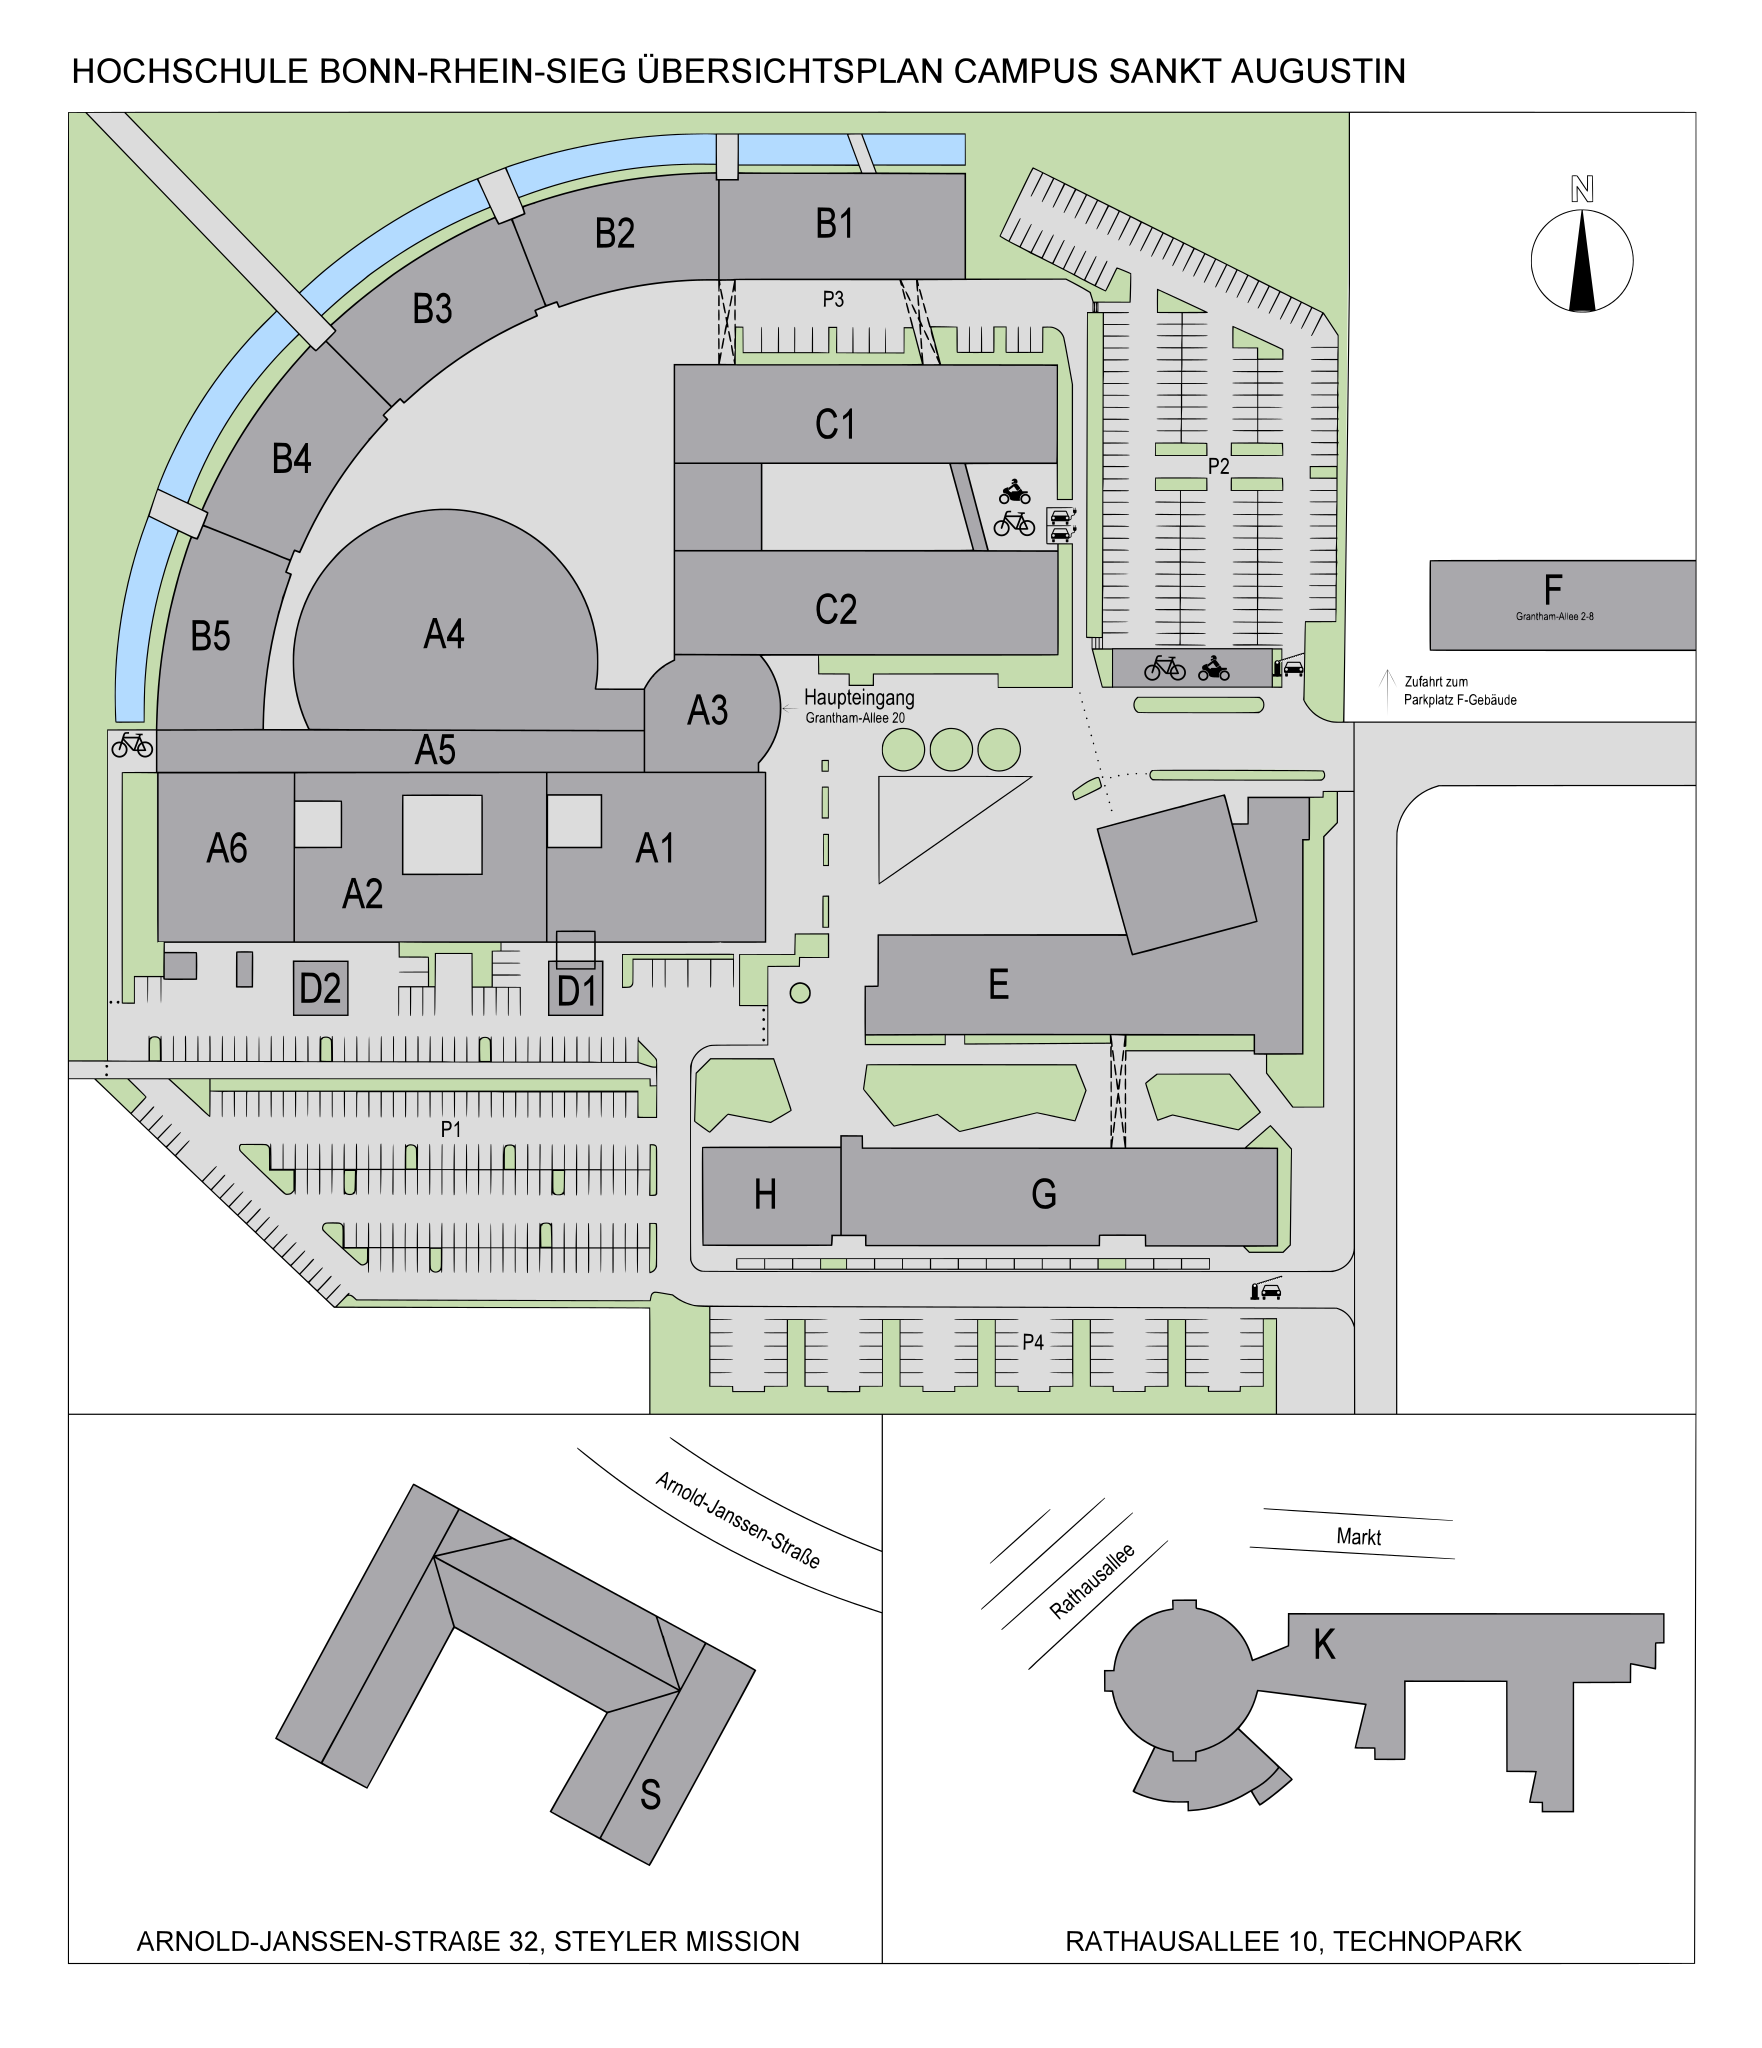
\includegraphics[width=0.95\textwidth]{./2.0.0.0_content/photos/campus/Lageplan-Campus-Sankt-Augustin-2025.png}
    \label{Dieser Lageplan fast aktuell.}
\end{figure}




\clearpage









% ---------------------------
% Wichtige Orte, Lernplätze und Portale
\PART{Wichtige Orte, Lernplätze und Portale}
% ---------------------------
    % \newpage
    % \section{Wichtige Orte Intern}

Hier findest du eine Übersicht über die wichtigsten Orte auf dem Campus Sankt Augustin, die dir den Studienalltag erleichtern.
\url{https://www.h-brs.de/de/inf/ansprechpartner-anlaufstellen}

\subsection{Fachschaft A051}
Natürlich der wichtigste Ort von allen: unser Büro \textbf{A051} der Fachschaft!

Du kannst bei uns bekommen:
\begin{itemize} [noitemsep,nolistsep]
    \item Ansprechpartner:innen für alle möglichen Fragen rund ums Studium
    \item Altklausuren (sofern vorhanden) \textbf{Nur mit USB-Stick oder SSD abholbar!}
    \item Drucker (kostenlos für Studierende vom FB02 im begrenzten Umfang)
    \item Getränke für 1€
    \item Kostenloses Wassereis
    \item Eine Couch zum Entspannen
    \item Einen Ort zum Treffen mit anderen Studierenden
\end{itemize}

Du findst uns direkt an der Hochschulstraße, geradeaus vom Haupteingang. Wir haben einen Bildschrim direkt vor dem Eingang des Büros mit aktuellen Events und Aktionen und den aktuellen Bahnfahrplan. Hier noch die Broadcastgruppen über WhatsApp und Signal.\\
\vspace{1mm}

\begin{flushleft}
  \qrcode[height=20mm]{https://chat.whatsapp.com/KhDfCdUPRx17hmxWPSGhqO?mode=ems_qr_t} \href{https://chat.whatsapp.com/KhDfCdUPRx17hmxWPSGhqO}{<--------\textbf{Whatsapp Broadcast}}
  \begin{flushright}
    \vspace{-23.5mm}
    \href{https://signal.group/#CjQKIANRh68V0_YvlDQHd29ezVVIEeYPAfFAK6zVbxDcsLMcEhBsm9SxVk57Vsyo5QniX0GT}{\textbf{Signal Broadcast}-------->}\qrcode[height=20mm]{https://signal.group/#CjQKIANRh68V0_YvlDQHd29ezVVIEeYPAfFAK6zVbxDcsLMcEhBsm9SxVk57Vsyo5QniX0GT}  
  \end{flushright}
\end{flushleft}



\subsection{Studierwerkstatt}

\vspace{-3mm}
\textbf{Studierwerkstatt, deine Anlaufstelle zum Lernen}
\vspace{-2mm}

Die \textbf{Studierwerkstatt} findest du in \textbf{Raum C153}. Hier bekommst du Unterstützung in fast allen \textbf{Grundlagenfächern der Informatik}. Ob Nachhilfe, Lernberatung oder einfach gemeinsames Lernen, hier bist du richtig.
\vspace{-2mm}

\textbf{Öffnungszeiten}  
In der Vorlesungszeit ist die Studierwerkstatt von Montag bis Freitag von \textbf{13:00 bis 19:00 Uhr} geöffnet.  
Kurz vor der zweiten Prüfungsphase sind die Zeiten \textbf{10:00 bis 12:00 Uhr} und \textbf{13:00 bis 17:00 Uhr}.
\vspace{-2mm}

\textbf{Wer hilft dir?}  
Das Angebot wird ausschließlich von Studierenden betreut, die als Studentischen Hilfskräfte(SHKs) oder wissenschaftliche Hilfskräfte(WHKs) angestellt sind.
\vspace{-2mm}

\textbf{Wie findest du die richtige Person?}  
Der \textbf{Arbeitsplan} hängt direkt in der Studierwerkstatt an einem Whiteboard. Dort kannst du sehen, wann Tutorinnen und Tutoren für dein Fach da sind.
\vspace{-2mm}

\textbf{Kosten}  
Der Service ist für dich komplett kostenlos.
\vspace{-2mm}

\textbf{Kontakt}  
\vspace{-2mm}

Komm einfach vorbei. Für organisatorische Fragen kannst du dich per Mail an \\
\href{mailto:oliver.lanzerath@h-brs.de}{oliver.lanzerath@h-brs.de} (Oliver Lanzerath) oder  
\href{mailto:sigrid.weil@h-brs.de}{sigrid.weil@h-brs.de} (Sigrid Weil) wenden.

\subsection{Mensa \& Koff-in vom STWB}
\subsubsection{\href{https://www.studierendenwerk-bonn.de/essen-trinken/mensen-cafes/mensa-sankt-augustin}{Mensa vom STWB}}

\vspace{-3mm}
Direkt links vom Haupteingang findest du die Mensa. Dort gibt es von \textbf{Montag} bis \textbf{Freitag} Mittagessen.  
Das aktuelle Menü siehst du an den \textbf{Monitoren} im \textbf{Eingang der Mensa}, \textbf{online beim Studierendenwerk} oder direkt \textbf{vor unserem Büro} auf dem \textbf{Bildschirm} mit dem Wochenplan oder weiter unten im Text über den \textbf{QR-Code}.\\
Wenn du dein Essen ausgesucht hast, kannst du an die \textbf{SB-Kassen} oder die besetzten Kassen gehen. Bezahlen kannst du aktuell nur noch mit \textbf{Kreditkarte oder Girokarte} oder an den \textbf{SB-Kassen} mit deinem \textbf{Studierendenausweis}. Deinen Studierendenausweis kannst du an den Mensa-Automaten mit Hilfe deiner Bankkarte aufladen. Bargeld wird nicht mehr akzeptiert.

\vspace{-2mm}
Außerhalb von Öffnungszeiten der Mensa wird der Speisesaal als Lernraum angeboten und während der Prüfungsphasen als Prüfungsraum genutzt.

\textbf{Öffnungszeiten Mo–Fr}
\vspace{-2mm}

\begin{itemize}[noitemsep,nolistsep]
  \item Während des Semesters: \textbf{11:30–14:30 Uhr}
  \item Vorlesungsfreie Zeit: \textbf{11:30–14:00 Uhr}
  \item Prüfungsphase: \textbf{11:30–14:00 Uhr}
\end{itemize}
\vspace{-4pt}

\begin{center}
  \qrcode[height=30mm]{https://www.maxmanager.de/daten-extern/sw-bonn/pdf/wochenplaene/1/aktuell_de.pdf}\\
  \vspace{5mm}
  \textbf{ Dieser QRcode zeigt euch \underline{IMMER} den aktuellen Wocheplan der Mensa}\\
  \small\url{https://www.maxmanager.de/daten-extern/sw-bonn/pdf/wochenplaene/1/aktuell_de.pdf}\\
  \vspace{5mm}
  \textbf{ Dieser QRcode zeigt euch \underline{IMMER} den nächsten Wocheplan der Mensa}\\
  \small\url{https://www.maxmanager.de/daten-extern/sw-bonn/pdf/wochenplaene/1/naechste-woche_de.pdf}\\
  \vspace{1mm}
  \qrcode[height=30mm]{https://www.maxmanager.de/daten-extern/sw-bonn/pdf/wochenplaene/1/naechste-woche_de.pdf}\\
\end{center}
\vspace{-4pt}

\textbf{Tipp:} Zwischen \textbf{12:00 Uhr und 13:00 Uhr} gibt es den größten Andrang. Gehe entweder direkt nach den Vorlesungen oder so spät wie möglich, damit du nicht zu lange in der Schlange warten musst und die Stoßzeiten umgehst.

\subsubsection{Koff-in vom STWB}
Geöffnet \textbf{Mo–Fr}:
\begin{itemize}[noitemsep,nolistsep]
  \item Im Semester: \textbf{\textbf{08:00–16:00} Uhr}
  \item In den Semesterferien: \textbf{\textbf{08:00–14:00} Uhr}
  \item Prüfungsphasen: \textbf{\textbf{08:00–15:00} Uhr}
\end{itemize}

Wenn dir der \textbf{Andrang an der Mensa} zu viel wird oder du \textbf{zwischen deinen Vorlesungen} eine Stärkung brauchst kannst du auch zum \textbf{koff-in} gehen. Das ist wie ein kleines Café mit halbrunder Theke und gemütlichen Sitzmöglichkeiten. 
Den findest du entlang der Hochschulstraße weiter runter, unmittelbar neben der Mensa.

Dort gibt es belegte Brötchen, Sandwiches, Backwaren, Müsli-Joghurts, Süßwaren, kalte Getränke wie Kakao, Softdrinks oder Energy Drinks und auch Heißgetränke.

Bring gerne deinen eigenen Becher für Heißgetränke mit, sonst gibt es auch die \textbf{LogiCups Becher} die du für einen Aufpreis für 0,70€ bekommen kannst, wenn du mal nicht vor Ort sitzen möchtest. Bei der Rückgabe des Bechers bekommst du \textbf{0,50€} als \textbf{Pfandrückgabe} wieder.

Gezahlt kann nur noch digital per Bankkarte, Debitkarte oder mit deinem Studiausweis den du vorab an den Mensa-Automaten aufladen kannst. Dein Studiausweis, kann dich nicht nur ausweisen, sondern auch für dich bezahlen! (aber (ausschließlich) an \textbf{allen Orten vom Studierendenwerk Bonn} (\href{https://www.studierendenwerk-bonn.de/essen-trinken}{\textbf{Mensen, Cafés}}))

\begin{center}
  \qrcode[height=30mm]{https://www.studierendenwerk-bonn.de/essen-trinken}\\
  \href{https://www.studierendenwerk-bonn.de/essen-trinken}{\textbf{https://www.studierendenwerk-bonn.de/essen-trinken}}
\end{center}

\textbf{Tipp:} Ab und zu gibt es frische Waffeln, schnell sein lohnt sich!

Sollte selbst das Koff-in zu Stoßzeiten mal überfüllt sein oder ist die Schlange zu lang, gibt es für Heißgetränke sogar eine dritte Alternative die du in der Hochschule finden kannst. 

\paragraph{CaffKar vom Café ``das Cultura``}

Dieser Wagen wird von \textbf{8:00 Uhr bis 16:00 Uhr} von Studierenden und gelegentlich ``vom Besitzer`` geführt/bedient. Finden kannst du ihn draußen neben dem Haupteingang oder am Ende der Hochschulstraße. \\
Dort bekommst du in den \textbf{RECUP Bechern} ebenfalls diverse Heißgetränke, die aufwändiger und sogar mit Extras zubereitet werden, wie z.B. Sirups. Für die Becher dort gibt es ebenfalls ein \textbf{Pfand von 1€} den du bei Rückgabe wieder \textbf{vollständig zurückbekommst}.  



\newpage
\subsection{Bibliothek}

\subsubsection*{Bibliothek für Erstis}
\vspace{-4mm}
\begin{wrapfigure}{r}{0.45\textwidth}
  \vspace{-10pt}
  \includegraphics[width=\linewidth]{./2.0.0.0_content/photos/Bib/Ausleihe und Rückgabe.jpg}
\end{wrapfigure}

Willkommen an der H-BRS und in der Bibliothek!  

In Sankt Augustin findest du die Bibliothek im Hauptgebäude A im 1. OG und in Rheinbach im 1. OG des C-Gebäudes.  

Dein Studierendenausweis ist gleichzeitig auch dein Bibliotheksausweis. Du kannst beide Bibliotheken nutzen.  
Falls ein Buch nicht vor Ort ist, kannst du es über den \textbf{Fernleihservice} bestellen.  




\medskip
\textbf{Logins:}
\vspace{-3mm}
\begin{itemize}[itemsep=2pt,parsep=0pt,topsep=0pt]
  \item Bibliotheksservices (BibDiscover, BibPrint, BibCloud, Gruppenräume): Bibliotheksnummer + MIA-Passwort
  \item LEA: Fachbereichskürzel + MIA-Passwort
  \item Ausleihe am Selbstverbucher: Bibliothekskarte + Ausleih-PIN
  \item WLAN H-BRS: \url{https://info.h-brs.de/de/wlan/h-brs}
\end{itemize}

\vspace{-3mm}

\medskip
\textbf{Angebote:}
\vspace{-3mm}
\begin{itemize}[itemsep=2pt,parsep=0pt,topsep=0pt]%[noitemsep]
  \item Beratung zum wissenschaftlichen Arbeiten
  \item Software (Zotero, SciFlow)
  \item Datenbanken für die Recherche
  \item Lernplätze und Gruppenräume
  \item Ausleihe von Technik (Powerbanks, Kabel, Laptops …)
  \item Scannen, Drucken und Kopieren
  \item OBRS (One-Button-Recording-Studio)
\end{itemize}

\vspace{5mm}

\begin{center}
  \begin{minipage}{0.7\textwidth}
    \centering
    \textbf{Webseite der Bibliothek}\\
    \vspace{1mm}
    \qrcode[height=35mm]{https://www.h-brs.de/de/bibliothek}\\
    \vspace{1mm}
    \url{https://www.h-brs.de/de/bibliothek}
  \end{minipage}
\end{center}


\clearpage
%\subsubsection*{Gebühren und Kosten}
%\begin{wrapfigure}{l}{0.45\textwidth}
%  \vspace{-10pt}
%  \includegraphics[width=\linewidth]{./2.0.0.0_content/photos/Bib/whiteboard.jpg}
%\end{wrapfigure}

\begin{wrapstuff}[type=figure, l, width=0.5\textwidth, top=1]
    \setlength{\abovecaptionskip}{8pt plus 3pt minus 2pt}
    \centering
    \includegraphics[width=\textwidth]{./2.0.0.0_content/photos/Bib/Bibliothek Gruppe Lernen Imagekampagne 2023-05-24 Lichtenscheid 005.JPG}
    \\[0.5em]
    {\small \paragraph{Zu spät abgegeben?}
  \begin{itemize}[itemsep=2pt,parsep=0pt,topsep=0pt]
    \item bis 10 Tage: \textbf{2 €}
    \item bis 20 Tage: \textbf{5 €}
    \item bis 30 Tage: \textbf{10 €}
    \item mehr als 30 Tage: \textbf{20 €}
  \end{itemize}}
\end{wrapstuff}

Für alle Studis der H-BRS ist die Nutzung der Bib \textbf{komplett kostenlos}.  
Externe Nutzer:innen zahlen ein Jahresentgelt von \textbf{10 €}  
(Ausnahme: Studierende an staatlichen Hochschulen NRW).  

Du kannst Bücher und Medien jeweils nur für \textbf{einen Monat} ausleihen. Achte daher bei deinen Ausleihen darauf, dass du die geliehenen Sachen rechtzeitig zurückgibst, um Gebühren zu vermeiden.\\


%  \paragraph{Zu spät abgegeben?}
%  \begin{itemize}[itemsep=2pt,parsep=0pt,topsep=0pt]
%    \item bis 10 Tage: \textbf{2 €}
%    \item bis 20 Tage: \textbf{5 €}
%    \item bis 30 Tage: \textbf{10 €}
%    \item mehr als 30 Tage: \textbf{20 €}
%  \end{itemize}

\vspace{8mm}
  \paragraph{Weitere mögliche Kosten:}
  \vspace{-0,5mm}
  \begin{itemize}[itemsep=2pt,parsep=0pt,topsep=0pt]
    \item Fernleihe: \textbf{1,50 €}
    \item Neuer Ausweis: \textbf{10 €}
    \item Verlust/Ersatz: \textbf{25 €}
    \item Kopien/Ausdrucke: \textbf{0,05 € pro Seite}
    \item Extra-Service (bibliographische Auskünfte): \textbf{45 €/h} (min. 15 €)
  \end{itemize}

\vspace{3mm}
\begin{center}
  \qrcode[height=2cm]{https://www.h-brs.de/de/bib/gebuehren-und-kosten}\\
  \small\url{https://www.h-brs.de/de/bib/gebuehren-und-kosten}
\end{center}
\medskip
\textbf{Nützliche Links:}
\vspace{-3mm}
\begin{multicols}{2}
\begin{itemize}[itemsep=3pt,parsep=0pt,topsep=0pt]
  \item LEA: \url{https://lea.hochschule-bonn-rhein-sieg.de}
  \item Beratung: \url{https://www.h-brs.de/de/bib/beratungsangebot}
  \item Gruppenräume: \url{https://rrs.bib.h-brs.de/}
  \item Fernzugriff: \url{https://www.h-brs.de/de/bib/fernzugriff}
  \item BibPrint: \url{https://bib-print.bib.h-brs.de/user}
  \item BibCloud: \url{https://bib-cloud.bib.hochschule-bonn-rhein-sieg.de/login}
\end{itemize}
\end{multicols}


\subsubsection*{Regelmäßige Veranstaltungen}
\vspace{-5mm}
\begin{itemize}[itemsep=2pt,parsep=0pt,topsep=0pt]
  \item BibLounge – Schulungen zu Arbeiten, KI und Lernstrategien:  
    \url{https://www.h-brs.de/de/bib/biblounge-termine-und-themen}
  \item LiteraturKlatsch – literarisches Miteinander:  
    \url{https://www.h-brs.de/de/bib/literatur-klatsch-themen-und-termine}
  \item Zu Gast auf dem Sofa – Autorenlesungen:  
    \url{https://www.h-brs.de/de/bib/zu-gast-auf-dem-sofa}
\end{itemize}


\clearpage
\subsection{Sekretariat Informatik}

Das \textbf{Fachbereichssekretariat Informatik} in \textbf{C101} ist erster Ansprechpartner des Fachbereichs Informatik.  
Es unterstützt bei organisatorischen Fragen zu Studium, Lehrveranstaltungen, Lehraufträgen oder mitarbeiterrelevanten Themen und stellt den Kontakt zum Dekanat her. Außerdem ist hier die Abgabe und Entgegennahme von Post möglich (wenn nicht am Empfang über die Poststelle oder im Postkasten erhalten).


\textbf{Kontaktzeiten:}

\vspace{-3mm}
\begin{itemize}[noitemsep, nolistsep]
  \item Montag bis Mittwoch: 09:00 -- 12:00 Uhr
  \item Donnerstag: 09:00 -- 16:30 Uhr
  \item Vorlesungsfreie Zeit: Montag -- Freitag: 09:00 -- 12:00 Uhr
\end{itemize}

\textbf{E-Mail:} \href{mailto:fb02.sekretariat@h-brs.de}{fb02.sekretariat@h-brs.de}\\
\textbf{Webseite:} \href{https://www.h-brs.de/de/inf/sekretariat-des-fachbereichs-informatik}{Fachbereichssekretariat Informatik Webseite}

\vspace{-5mm}

\subsubsection*{Mitarbeiterinnen}

\begin{table}[!h]
\centering
\resizebox{\textwidth}{!}{%
\begin{tabular}{|l|l|l|l|l|}
\hline
\textbf{Name} & \textbf{Rolle} & \textbf{E-Mail} & \textbf{Raum} & \textbf{Telefon}  \\ \hline
Anne Maria Kaiser & Sekretariat & \href{mailto:anne.kaiser@h-brs.de}{\texttt{anne.kaiser@h-brs.de}} & C 101 & +49 2241 865 201 \\ \hline
Irina Malsam & Sekretariat & \href{mailto:irina.malsam@h-brs.de}{\texttt{irina.malsam@h-brs.de}} & C 101 & +49 2241 865 195 \\ \hline
Anette Schiffmann & Assistenz im Dekanat & \href{mailto:anette.schiffmann@h-brs.de}{\texttt{anette.schiffmann@h-brs.de}} & C 101 & +49 2241 865 201 \\ \hline
Kathrin Fetkenhauer & Assistenz der Prüfungsausschüsse & \href{mailto:kathrin.fetkenhauer@h-brs.de}{\texttt{kathrin.fetkenhauer@h-brs.de}} & C 105 & +49 2241 865 290 \\ \hline
\end{tabular}%
}
\end{table}



\vspace{-3mm}

\subsection{Empfang, Poststelle und Post}
\vspace{-1mm}

\subsubsection{Empfang}

\vspace{-4mm}
Der Empfang ist direkt geradeaus durch den Haupteingang in einem vitrinenähnlichen Häuschen.  
Dort kannst du:

\vspace{-4mm}
\begin{itemize}[itemsep=3pt, parsep=0pt, topsep=2pt]
  \item Schlüssel für Lernräume (über \textbf{SARBS} Online gebucht) abholen,
  \item deinen Studierendenausweis abholen,
  \item Fragen zu Räumen und Raumbuchungen stellen,
  \item Post abholen, über die Poststelle
  \item deine Fundsachen abholen (sofern sie dort abgegeben wurden).
\end{itemize}

\vspace{-2mm}
Der Empfang ist \textbf{bis 18 Uhr} besetzt. Danach übernimmt der Sicherheitsdienst: dann kannst du nur noch Schlüssel zurückgeben oder Briefe/Umschläge abgeben, die ggf. erst am nächsten Tag \textbf{gestempelt} werden.
\vspace{-5mm}

\subsubsection{Poststelle / Post}

\vspace{-2mm}
Die Poststelle ist von \textbf{7:30 Uhr} bis \textbf{15:30 Uhr} über den Empfang erreichbar. Dort kannst du von morgens bis \textbf{18 Uhr} Briefe, Pakete und andere Post abgeben. \textbf{(Sa-So geschlossen)}
Alternativ kannst du Briefe \textbf{links} neben dem Empfang einwerfen.  
Für Professor:innen gibt es Fächer direkt \textbf{vor dem Sekretariat} und \textbf{gegnüber an der Wand} im Flur.  
Am Empfang abgegebene Post \textbf{wird gestempelt}. Für \textbf{zeitkritische} Sendungen ist die Abgabe dort sinnvoller.  
Der Briefkasten vor dem Eingang wird \textbf{morgens} und \textbf{meist kurz vor Schließung} der Poststelle geleert.


\clearpage
\subsection{Servicepoint Fachbereich Informatik}
\textbf{\url{https://faq.infcs.de/servicepoint/}}

Wir sind die erste Anlaufstelle bei Problemen mit der \textbf{technischen Infrastruktur} des Fachbereichs.  

\medskip

\noindent
\textbf{Beispiele:}
\begin{itemize}[noitemsep,nolistsep]
  \item Ihr könnt euch in einen Account nicht mehr einloggen?
  \item Ein Upload-Portal funktioniert nicht wie erwartet?
  \item Ihr möchtet von zu Hause aus auf das Hochschul-Netzwerk zugreifen?
\end{itemize}

Außerdem unterstützen wir den \textbf{reibungslosen Ablauf des Studienbetriebs}.  

\medskip

\noindent
\textbf{Typische Fälle:}
\begin{itemize}[noitemsep,nolistsep]
  \item Ein Rechner in den Seminarräumen ist defekt.  
  \item Eure Lerngruppe möchte einen Raum leihen.  
  \item Dozent:innen kommen nicht mit der Raumtechnik klar.  
  \item Ihr müsst einen Vortrag halten, könnt euren Laptop aber nicht mit dem Beamer verbinden.  
\end{itemize}


In all diesen Situationen leisten wir \textbf{Soforthilfe}.\\
\vspace{5pt}
\textbf{Wofür können Studierende sich an uns wenden:}
\begin{itemize}[noitemsep,nolistsep]
  \item Einrichtung von \textbf{WLAN}, \textbf{VPN} und anderen Hochschuldiensten\\
  Wir unterstützen bei allen gängigen Geräten und Betriebssystemen, solange es das Studium betrifft!
  \item Probleme mit Hochschulaccounts:
  \begin{itemize}
    \item Welcher Account für welchen Dienst?
    \item Passwort vergessen?
  \end{itemize}
  \item Verleih von:
  \begin{itemize}
    \item Adaptern und Kabeln
    \item Seminarräumen für Lerngruppen
    \item Whiteboardmarkern und -reinigern
  \end{itemize}
\end{itemize}
Wie sind wir zu erreichen:
Werktags von \textbf{08:00 bis 18:00} in Raum \textbf{A102.1} (direkt über dem Haupteingang)
Oder per Mail an \href{mailto:servicepoint@mail.inf.h-brs.de}{\textbf{servicepoint@mail.inf.h-brs.de}}

\textbf{Tipps:} für einen guten Start ins Studium:
Macht euch direkt zum Start mit den Hochschulservices vertraut; nicht erst 5 Minuten vor der
ersten Abgabe. \text{;)}


    \newpage
    \section{Wichtige Orte Extern}

\subsection{Studierendenwerk Bonn}

\subsubsection{Psychologische Beratungsstelle (PBS)}
\vspace{-4mm}
Wenn dir im Studium mal alles zu viel wird, du mit Ängsten, Überforderung oder persönlichen Problemen kämpfst, kannst du dich an die \textbf{Psychologische Beratungsstelle (PBS)} des Studierendenwerks Bonn wenden.  
Die Gespräche sind \textbf{vertraulich, kostenlos} und richten sich speziell an Studierende der H-BRS.  
Es gibt Einzelgespräche, offene Sprechstunden sowie Online- oder Telefontermine.  

\textbf{Adresse:} Adenauerallee 63, 53113 Bonn
\textbf{Standort Sankt Augustin:} Raum E221 (Termine vorher online einsehen) \\
\qrcode[height=20mm]{https://www.studierendenwerk-bonn.de/beratung-soziales/psychologische-beratungsstelle-pbs}
\href{https://www.studierendenwerk-bonn.de/beratung-soziales/psychologische-beratungsstelle-pbs}{https://www.studierendenwerk-bonn.de/beratung-soziales/pbs}
\vspace{-4mm}

\subsubsection{Schreibberatung}
\vspace{-4mm}
Wenn du Unterstützung beim Schreiben deiner Haus- oder Abschlussarbeit brauchst oder Hilfe im Umgang mit Schreibblockaden suchst, kannst du die \textbf{Schreibberatung} nutzen.  
Du bekommst individuelles Feedback zu deinem Schreibprozess und zur Struktur deiner Texte.  
Es gibt auch eine \emph{offene Schreibberatung} in der Universitäts- und Landesbibliothek.  

\textbf{Adresse:} Adenauerallee 63 / 39-41, 53113 Bonn \\
\qrcode[height=20mm]{https://www.studierendenwerk-bonn.de/beratung-soziales/schreibberatung}
\href{https://www.studierendenwerk-bonn.de/beratung-soziales/schreibberatung}{https://www.studierendenwerk-bonn.de/beratung-soziales/schreibberatung}
\vspace{-4mm}

\subsubsection{Finanzielle Hilfe}
\vspace{-4mm}
\paragraph{BAföG}
Wenn du dein Studium mit \textbf{BAföG} finanzieren möchtest, ist das Studierendenwerk Bonn deine Anlaufstelle.  
Dort bekommst du Unterstützung bei der Antragstellung, bei Fragen zur Förderhöhe, Anrechnung von Einkommen, Auslandsförderung oder Hilfe zum Studienabschluss.  

\textbf{Adresse:} Lennéstraße 3, 53113 Bonn \\
\qrcode[height=20mm]{https://www.studierendenwerk-bonn.de/finanzieren}
\url{https://www.studierendenwerk-bonn.de/finanzieren}




\clearpage
\paragraph{Freitisch}

Falls es mit dem Geld knapp ist, kannst du mit dem \textbf{Freitisch} kostenlos in der Mensa essen.  
Montag bis Freitag (außer an Feiertagen) gibt es morgens belegte Brötchen und ein Getränk, mittags ein Hauptgericht mit Beilagen und Getränk (auch Food-Truck möglich), und nachmittags ein Angebot aus der Cafeteria.  
\begin{flushright}
  \url{https://www.studierendenwerk-bonn.de/beratung-soziales/freitisch}
  \qrcode[height=20mm]{https://www.studierendenwerk-bonn.de/beratung-soziales/freitisch}
\end{flushright}



\paragraph{Darlehen und Kredite}

Neben BAföG kannst du mit Unterstützung des BAföG-Amts auch auf Darlehen und Kredite zurückgreifen:  

\begin{itemize}[noitemsep,nolistsep]
  \item Daka-Darlehen
  \item BMBF-Bildungskredit
  \item Hilfe zum Studienabschluss
\end{itemize}
\begin{flushright}
  \url{https://www.studierendenwerk-bonn.de/finanzieren/studienkredite}
  \qrcode[height=20mm]{https://www.studierendenwerk-bonn.de/finanzieren/studienkredite}
\end{flushright}

\paragraph{Stipendien}

\textbf{Stipendien} sind finanzielle Förderungen, die du nicht zurückzahlen musst.  
Sie werden nicht nur für gute Noten vergeben, sondern auch für Engagement, besondere Lebensumstände oder deinen Werdegang.  
Ein Stipendium kann dir den finanziellen Druck nehmen und neue Freiräume schaffen.  


\begin{itemize}[itemsep=3pt,parsep=0pt,topsep=0pt]
  \item \url{https://www.stipendiumplus.de} – 13 große Begabtenförderwerke
  \item \url{https://www.stipendienlotse.de} – offizielle Datenbank vom BMBF
  \item \url{https://www.e-fellows.net} – über 800 Stipendienprogramme
  \item \url{https://www.elfi.info} – Rechercheportal für Fördermöglichkeiten
  \item \url{https://www.auslandsstipendien.de} – speziell für Auslandsförderung
  \item \url{https://www.stiftungssuche.de} – über 10.000 Stiftungen
  \item \url{https://www.deutsches-stiftungszentrum.de} – wissenschaftsnahe Stiftungen
  \item \url{https://www.maecenata.eu} – bundesweite Stiftungsdatenbank
  \item \url{https://www.deutschlandstipendium.de} – einkommensunabhängige Förderung
  \item \url{https://www.aufstiegsstipendium.de} – für Berufserfahrene im Studium
  \item \url{https://www.arbeiterkind.de/studium-finanzieren/stipendien} – Extra für Arbeiterkinder
\end{itemize}

\par\vspace{-7mm}


\clearpage
\subsubsection{Studieren mit Kind}
\paragraph{BAföG mit Kind}

Studierende mit Kind können im Rahmen des BAföG einen \textbf{Kinderbetreuungszuschlag} erhalten: \textbf{130\,€ pro Kind unter 10 Jahren}, zusätzlich zur regulären Förderung.  

Außerdem kann BAföG auch über die übliche Altersgrenze von 30 Jahren hinaus gewährt werden, wenn die Pflege und Erziehung des Kindes ursächlich für die Überschreitung waren.  

\qrcode[height=20mm]{https://www.uni-bonn.de/de/universitaet/chancengerechtigkeit/familiengerechte-hochschule/studium-und-familie/finanzierung}
\url{https://www.uni-bonn.de/de/universitaet/chancengerechtigkeit/familiengerechte-hochschule/studium-und-familie/finanzierung}

\paragraph{Kindertagesstätte und Angebote}

Wenn du mit Kind am Campus Sankt Augustin studierst, kannst du die \textbf{Kindertageseinrichtung des Studierendenwerks} nutzen (Europaring 86). Dort werden rund 30 Kinder bis zum Schuleintritt betreut, %auch mit Plätzen für Studierende der H-BRS.  

Außerdem gibt es \textbf{Familienwohnungen} im Wohnheimen (mit Wohnberechtigungsschein) sowie den \emph{„Bonnapetit“-Kinderteller} in der Mensa, der Kindern eine kostenlose Mahlzeit ermöglicht.

Zusätzlich unterstützt dich die Hochschule mit dem Beratungsangebot \textbf{HELP}, das dir bei allen Fragen rund um Studium und Familie zur Seite steht. (Betreuung, Urlaubssemester, Eltern-Kind-Arbeitsplätze, Nothilfefonds).   

\qrcode[height=20mm]{https://www.studierendenwerk-bonn.de/studieren-mit-kind/}
\url{www.studierendenwerk-bonn.de/studieren-mit-kind/}

\vspace{7pt}
\textbf{Tipp:} Auf dem Hochschulgelänge, bzw. im Innenhof der Hochschule gibt es sogar einen Spielplatz den die Kinder von den Studierenden der H-BRS nutzen können.

\clearpage
\paragraph{Windelgeld}

Studierende der H-BRS und Universität Bonn können \textbf{einmal pro Kind unter 6 Jahren} ein Windelgeld beantragen: \textbf{200\,€} in einer Summe pro Semester.  

Anspruchsberechtigt sind Studierende mit geringem Einkommen, die keine anderen Leistungen wie BAföG (Abschnitt II), Daka-Darlehen oder KfW-Studienkredit beziehen und deren Nettoeinkommen nach Abzug von Miete und Versicherung unter einer bestimmten Schwelle liegt.  

Das Windelgeld hilft, die ersten Kosten (z.\,B. Windeln, Ausstattung) abzufedern, wenn die Finanzierung knapp ist.  

\begin{flushright}
  \url{https://www.studierendenwerk-bonn.de/beratung-soziales/windelgeld}
  \qrcode[height=20mm]{https://www.studierendenwerk-bonn.de/beratung-soziales/windelgeld}
\end{flushright}


\paragraph{Beratungsangebot - Studieren mit Kind}

Das „Studieren mit Kind“-Programm des Studierendenwerks Bonn bietet \textbf{flexible Kinderbetreuung}, unter anderem über \textbf{KinderSt.E.R.N.}, ein stundenweises Angebot am Nachmittag oder Abend.  

Zusätzlich gibt es \textbf{Kitaplätze} an mehreren Standorten (Bonn, Sankt Augustin, Rheinbach) mit ganztägiger Betreuung, teils in Kooperation mit der Universität und der Hochschule.  

Die Beratung umfasst Hilfe bei Organisation, Vereinbarkeit, Finanzierung und Betreuungsmöglichkeiten für studierende Eltern.


\begin{flushright}
  \url{www.studierendenwerk-bonn.de/studieren-mit-kind/}
  \qrcode[height=20mm]{https://www.studierendenwerk-bonn.de/studieren-mit-kind/}
\end{flushright}




    % \newpage
    % \input{2.0.0.0_content/pages/lernplätze.tex}
    % \newpage
    % \input{2.0.0.0_content/pages/portale.tex}


% ---------------------------
% Hochschulgruppen & Vereine
% \PART{Hochschulgruppen \& Vereine}
% % ---------------------------
%     \newpage
%     \input{2.0.0.0_content/pages/gruppen_vereine.tex}



% ---------------------------
% Gremien & Beratung
% \PART{Gremien \& Beratung}
% % ---------------------------
%     \newpage
%     \input{2.0.0.0_content/pages/asta.tex}
%     \newpage
%     \input{2.0.0.0_content/pages/stupa.tex}
%     \newpage
%     \section{Wahlen}

\subsection{Gremienwahlen}
An der Hochschule Bonn-Rhein-Sieg finden regelmäßig Wahlen für die studentische Selbstverwaltung statt.  
Studierende können wählen und selbst kandidieren.

\subsection*{Studentische Selbstverwaltung}
\begin{itemize}[noitemsep,nolistsep]
  \item \textbf{Fachschaftsräte} – gewählte Vertretung auf Fachbereichsebene nach § 53 HG NRW.  
  Sie vertreten die Interessen der Studierenden im Fachbereich, wirken in Gremien mit und organisieren Angebote wie Erstsemester-Einführungen, Lernmaterialien oder Veranstaltungen.  
  Für dich sind sie die direkten Ansprechpartner:innen im Studienalltag, z. B. bei Fragen zu Modulen, Problemen mit Prüfungen oder der Suche nach Mitstudierenden für Projekte oder leiten an die richtige stelle weiter.

  \item \textbf{Studierendenparlament (StuPa)} – nach § 53 HG NRW das \emph{höchste beschlussfassende Organ} der Studierendenschaft.  
  Es entscheidet über die Verwendung der Semesterbeiträge in Ordnugnen, erlässt Satzungen und legt die Grundlinien studentischer Hochschulpolitik fest.  
  Als Student:in profitierst du davon, dass über Finanzen (z. B. Semesterticket, Kulturförderung) transparent und demokratisch entschieden wird und deine Interessen auf Hochschulebene gebündelt werden.  

  \item \textbf{Allgemeiner Studierendenausschuss (AStA)} – die Exekutive der Studierendenschaft.  
  Er setzt die Beschlüsse des StuPa um, vertritt die Studierenden nach außen und bietet konkrete Services wie das Semesterticket, Beratungsangebote (Soziales, Recht, Internationales) oder Kultur- und Sportveranstaltungen.  
  Für dich bedeutet das: Der AStA ist deine Service- und Beratungsstelle, die dir bei Alltagsproblemen hilft und dein Studium durch zusätzliche Angebote bereichert.  
\end{itemize}

\subsection*{Studentische Wahlen im Detail}
\begin{itemize}[noitemsep,nolistsep]
  \item \textbf{Fachschaftswahlen}
  Jeder Fachbereich hat eine Fachschaft(alle volleingeschriebenen Studierenden) und diese einen Fachschaftsrat, die die Ersti-Woche, Events, Partys und Beratungen organisiert und deine Interessen vertritt.  
  \textbf{Wahlen:} jährlich; alle Studierenden des Fachbereichs dürfen wählen und kandidieren.

  \item \textbf{StuPa-Wahlen}
  Das \textbf{Studierendenparlament (StuPa)} entscheidet über Finanzen durch den Haushaltsauschuss, studentische Projekte und Positionen gegenüber der Hochschule.  
  \textbf{Wahlen:} jährlich; wahlberechtigt sind alle Studierenden der Hochschule.

  \item \textbf{AStA}
  Der \textbf{Allgemeine Studierendenausschuss (AStA)} setzt StuPa-Beschlüsse um, vertritt die Studierenden nach außen und bietet Services.  
  \textbf{Wahl:} nicht direkt; das StuPa wählt den AStA nach jeder Wahlperiode neu.
\end{itemize}

\subsection*{Wahlturnus}
\begin{itemize}
  \item Studentische Gremien: jährlich  
\end{itemize}


\subsection*{Warum wählen?}
Mit deiner Stimme entscheidest du, wer deine Interessen gegenüber Hochschule und Politik vertritt.  
Ob Semesterticket, Prüfungsordnungen oder Beratungsangebote, überall stecken gewählte Studierende dahinter.

\vspace{2em}

\subsection{Hochschulwahlen}
Hochschulwahlen betreffen die akademische Selbstverwaltung.  
Hier werden z. B. Vertreter:innen für den \textbf{Senat}, die \textbf{Fachbereichsräte} und Studierendenplätze im \textbf{Hochschulrat} bestimmt.  
Diese Gremien treffen Entscheidungen zu Lehre, Studium, Prüfungsordnungen und der strategischen Ausrichtung der Hochschule.

\subsection*{Akademische Selbstverwaltung}
\begin{itemize}
  \item \textbf{Senat} – das zentrale Gremium der Hochschule.  
  Er entscheidet über die Prüfungsordnungen, Studienordnungen und alle Grundsatzfragen von Studium und Forschung.  
  Im Senat sind auch Studierende vertreten, sodass du direkt Einfluss auf hochschulweite Regelungen und Entwicklungen nehmen kannst.  

  \item \textbf{Fachbereichsräte} – die Parlamente der einzelnen Fachbereiche.  
  Sie beschließen über Lehr- und Forschungsinhalte, die Organisation der Studiengänge und die Verteilung von Ressourcen im Fachbereich.  
  Für dich bedeutet das: Hier kannst du über die Ausgestaltung deines Studiums und die Weiterentwicklung deines Fachs mitentscheiden.  

  \item \textbf{Hochschulrat} – das strategische Kontroll- und Beratungsgremium der Hochschule.  
  Er überwacht die wirtschaftliche Lage, übt die Aufsicht über die Geschäftsführung aus, beschließt den Entwicklungsplan und berät Präsidium und Senat in Grundsatzfragen.  
  Auch wenn der Hochschulrat eher auf einer übergeordneten Ebene arbeitet, können diese an der strategische Ausrichtung der Hochschule mitgestalten.  
\end{itemize}


\subsection*{Wahlturnus}
\begin{itemize} 
  \item Senat und Fachbereichsräte: alle zwei Jahre  
  \item Hochschulrat: alle fünf Jahre (Bestellung, keine klassische Wahl)  
\end{itemize}


\subsection*{Warum wählen?}
Mit deiner Stimme entscheidest du, wer deine Interessen gegenüber Hochschule und Politik vertritt.  
Ob Semesterticket, Prüfungsordnungen oder Beratungsangebote, überall stecken gewählte Studierende dahinter.


%     \newpage
%     \input{2.0.0.0_content/pages/fachbereichsgremien.tex}
%     \newpage
%     \input{2.0.0.0_content/pages/hochschulgremien.tex}
%     \newpage
%     \section{Vertrauenspersonen}

Sie sind zentrale Ansprechpartner:innen für Studierende, Mitarbeitende und Lehrende des Fachbereichs Informatik, insbesondere in herausfordernden Situationen. 
Das Ziel ist es, ein sicheres, offenes und unterstützendes Umfeld an der Hochschule zu schaffen.

\subsection*{Hochschulmitarbeitende}

Diese Vertrauenspersonen sind im Fachbereich Informatik tätig:

\begin{table}[!h]
\centering
\resizebox{\textwidth}{!}{%
\begin{tabular}{|l|l|l|l|l|}
\hline
\textbf{Name} & \textbf{Rolle} & \textbf{E-Mail} & \textbf{Raum} & \textbf{Telefon}  \\ \hline
Prof. Dr. Alexandra Kees & Professorin & \texttt{alexandra.kees@h-brs.de} & C 220 & Tel: +49 2241 865 237  \\ \hline
Stephan Baum  & Mitarbeiter  & \texttt{stephan.baum@h-brs.de}  & C 161 & Tel: +49 2241 865 243 \\ \hline
Javed Razzaq, M.Sc.  & Mitarbeiter  & \texttt{javed.razzaq@h-brs.de}  & C 160 & Tel: +49 2241 865 231 \\ \hline
Dr. Mirko Seithe  & Lehrkraft  & \texttt{mirko.seithe@h-brs.de}  & C 182 & Tel: \\ \hline
Pia Barion  & SHK  & \texttt{pia.barion@h-brs.de}  & E 304 & Tel:\\  \hline
Miriam Kist, B.Sc.   & Mitarbeiterin   & \texttt{miriam.kist@h-brs.de}  & C 157 & Tel: +49 2241 865 789 \\ \hline
\end{tabular}%
}
\end{table}

\subsection*{Studentische Vertrauenspersonen}
Diese Vertrauenspersonen sind Studierende des Fachbereichs Informatik und arbeiten in der Fachschaft mit:

\begin{table}[!h]
\centering
\resizebox{\textwidth}{!}{%
\begin{tabular}{|l|l|l|l|l|}
\hline
\textbf{Name} & \textbf{Rolle} & \textbf{E-Mail} & \textbf{Raum} & \textbf{Telefon} \\ \hline
Jannik Hofmann & Studentische Vertrauensperson & \texttt{feedback-fs-inf@h-brs.de} & A 051 & Tel:+49 2241 865 662 \\ \hline
Lisa Höfges & Studentische Vertrauensperson & \texttt{feedback-fs-inf@h-brs.de} & A 051 & Tel:+49 2241 865 662 \\ \hline
\end{tabular}%
}
\end{table}

%     \newpage
%     \input{2.0.0.0_content/pages/studierendenberatung.tex}
%     \newpage
%     \input{2.0.0.0_content/pages/studierendenservice.tex}
%     \newpage
%     \input{2.0.0.0_content/pages/respekt.tex}
%     \newpage
%     \input{2.0.0.0_content/pages/raumderstille.tex}
%     \input{2.0.0.0_content/pages/help_Beratung.tex}

% ---------------------------
% Prüfungen, Prüfungsordnung und Curriculum
%\PART{Prüfungen, Prüfungsordnung und Curriculum}
% ---------------------------

    %\newpage
    %\input{2.0.0.0_content/pages/prüfungen_nta.tex}

    
    %\newpage
    %\input{2.0.0.0_content/pages/curriculum1.tex} %Kurz Version für Print
    %\input{2.0.0.0_content/pages/curriculum2.tex} %Lang Version für PDF
    %\newpage
    %\input{2.0.0.0_content/pages/prüfungsordnung.tex} %Lang Version für PDF
    %\includepdf[pages=-]{./3.0.0.0_other_content/pos_inf_2024_2025.pdf}
    %\input{2.0.0.0_content/pages/änderungsordnung.tex} %Zukünfig für Übergangsordnung nicht mehr in Ersti-Heft28 anhängen
    %\includepdf[pages=-]{./3.0.0.0_other_content/pos_inf_2024_2025_übergangsordnung.pdf}
    

% ---------------------------
% % Semesterticket
% \PART{Semesterticket}
% % ---------------------------
%     \newpage
%     \input{2.0.0.0_content/pages/semesterticket.tex}


% ---------------------------
% VPN, WLAN und Service
% \PART{VPN, WLAN, Office 365 und Service}
% % ---------------------------

%     \newpage
%     \section{VPN, Cloud, Office 365 und Service}

\begin{enumerate}[label*=\arabic*.,noitemsep,nolistsep]
    % VPN und Proxy
    \item \textbf{VPN und Proxy}
    \begin{enumerate}[label*=\arabic*.]
        \item \textbf{Proxy für FB02 und akademische Software}  
        Zugriff auf interne Systeme des Fachbereichs ist möglich, \textbf{VPN wird empfohlen}.  
        \begin{itemize}[left=1em]
            \item Proxy-PAC: \href{http://proxypac.inf.h-brs.de/proxy.pac}{proxypac.inf.h-brs.de/proxy.pac}
            \item HTTP-Proxy: \href{http://www-cache.inf.h-brs.de:8080}{www-cache.inf.h-brs.de:8080} oder \href{http://10.20.204.15:8080}{10.20.204.15:8080}
            \item Kein Zugriff auf die Bibliothek über diesen Proxy
            \item \textcolor{blue}{Empfohlen:} iOS, Mac, Windows
            \item \textcolor{red}{Nicht empfohlen:} Android, Linux (komplizierte Einrichtung, langsame Verbindung)
        \end{itemize}

        \item \textbf{VPN Tunnel mit OpenVPN}  
        Der Fachbereich stellt einen eigenen VPN-Server bereit.  
        \begin{itemize}[left=1em]
            \item Download: \href{https://portal.inf.h-brs.de/certmk/}{Configs, Zertifikate, Schlüssel}
            \item Empfohlene Plattformen: Android, Windows, Linux, Mac
            \item Android: App \href{https://play.google.com/store/apps/details?id=de.blinkt.openvpn}{OpenVPN für Android} verwenden
            \item iOS: nicht empfohlen (nur eine VPN-Verbindung gleichzeitig; Proxy parallele Nutzung besser)
        \end{itemize}

        \item \textbf{VPN zur Bibliothek / Fernzugriff}  
        Für Bibliothekszugriff empfohlen, besonders wenn kein VPN für FB02 benötigt wird.  
        \begin{itemize}[left=1em]
            \item Proxy für Bibliothek: \href{https://www.h-brs.de/files/proxy.pac}{proxy.h-brs.de}
            \item Infos \& Anleitung: \href{https://www.h-brs.de/de/bib/fernzugriff}{Fernzugriff Info}
            \item Konfigurationen:
            \begin{itemize}
                \item Windows 10: \href{https://www.h-brs.de/de/bib/fernzugriff-konfiguration-windows-10}{Anleitung}
                \item Firefox: \href{https://www.h-brs.de/de/bib/fernzugriff-konfiguration-mozilla-firefox}{Anleitung}
                \item Mac OS: \href{https://www.h-brs.de/de/bib/fernzugriff-konfiguration-safari}{Anleitung}
                \item iPad: \href{https://www.h-brs.de/de/bib/konfiguration-ipad-fuer-den-fernzugriff}{Anleitung}
                \item FAQ: \href{https://www.h-brs.de/de/bib/haeufig-gestellte-fragen-zum-fernzugriff}{Häufig gestellte Fragen}
            \end{itemize}
        \end{itemize}
    \end{enumerate}
    % Systeme und Dienste
    \item \textbf{Systeme und Dienste}
    \begin{enumerate}[label*=\arabic*., left=1em]
        \item \textbf{Cloudspeicher}
        \begin{itemize}[left=1em]
            \item \textbf{H-BRS Sciebo} (30 GB)  
            Registrierung notwendig, ähnlich wie Nextcloud oder ownCloud.  
            \begin{itemize}
                \item Beispielkennung: \texttt{mmuste2s@h-brs.de}
                \item Weblogin: \href{https://h-brs.sciebo.de/login}{https://h-brs.sciebo.de/login}
                \item Verwaltung: \href{https://www.sciebo.de/mysciebo_uebersicht}{My.Sciebo}
                \item Dokumenteneditor für Text, Tabellen, Präsentationen
                \item Apps für PC \& Smartphone: \href{https://www.sciebo.de/de/download}{Download}
                \item Hilfe: \href{https://www.sciebo.de/de/hilfe}{Anleitung}
                \item Kontakt: \href{https://www.sciebo.de/de/kontakt/index.html}{Kontaktformular}
                \item Account gültig für 12 Monate, verlängerbar solange Mitglied einer Einrichtung
                \item Verbindung mit Nextcloud-Apps möglich
            \end{itemize}
            \item \textbf{BIB-Cloud:} 15 GB Speicher
            \begin{itemize}
                \item Account existiert solange du an der Hochschule immatrikuliert bist. Keine Erstellung notwendig
                \item Weblogin: \href{https://bib-cloud.bib.hochschule-bonn-rhein-sieg.de}{https://bib-cloud.bib.hochschule-bonn-rhein-sieg.de}
                \item Bibliotheksnummer + MIA-Passwort
                \item Verbindung mit Nextcloud-Apps möglich \url{https://nextcloud.com/}
            \end{itemize}
        \end{itemize}
    \end{enumerate}
    \item \textbf{Service}
    \begin{enumerate}
        \item \textbf{Servicepoint Fachbereich Informatik}
        \begin{itemize}[noitemsep,nolistsep]
            \item \textbf{Technische Infrastruktur:} Hilfe bei Account-Problemen, Passwörtern, WLAN, VPN und Zugängen zu Hochschuldiensten.  
            \item \textbf{Studienbetrieb:} Unterstützung bei defekten Rechnern, Raumtechnik, Beamerproblemen und Raumverleih für Lerngruppen.  
            \item \textbf{Geräte- und Materialverleih:} Adapter, Kabel, Whiteboardmarker und mehr.  
            \item \textbf{Erreichbarkeit:} Werktags 08:00–18:00 in A102.1 \\ oder per Mail an \href{mailto:servicepoint@mail.inf.h-brs.de}{servicepoint@mail.inf.h-brs.de}.  
            \item \textbf{Tipp:} Macht euch frühzeitig mit den Hochschulservices vertraut, um Stress vor Abgaben zu vermeiden.  
        \end{itemize}
        \item \textbf{LEA-Support für Informatik}
        \begin{itemize}[noitemsep,nolistsep]
            \item \textbf{Zuständigkeit:} Für den Fachbereich Informatik ist \textbf{Melanie Klöß} deine Ansprechpartnerin im E-Learning-Team. 
            \item \textbf{Service:} Sie unterstützt dich beim administrativen LEA-Support und bei allen Fragen rund um digitale Lehre und E-Prüfungen. 
            \item \textbf{Raum:} A 167 
            \item \textbf{Tel:} +49 2241 865 788
            \item \textbf{Mail:} \href{mailto:melanie.kloess@h-brs.de}{melanie.kloess@h-brs.de}
            \item \textbf{Webseite:} \url{https://www.h-brs.de/de/elearning/kontakt}.  
        \end{itemize}
        \item \textbf{Druckpunkt – Dein Copyshop an der H-BRS}
        \begin{itemize}[noitemsep,nolistsep]
            \item \textbf{Abschlussarbeiten drucken und binden} (Hardcover, Softcover, Spiralbindung) sowie Poster, Plakate und Großformate.  
            \item \textbf{Schnell und direkt auf dem Campus} – Expressdruck möglich.  
            \item \textbf{Weitere Services:} Scans, Bildbearbeitung, Geschäftspapiere, Visitenkarten.  
            \item \textbf{Kontakt:} Grantham-Allee 20, Mo–Do 8:30–16:00, Fr 8:30–15:00, 
            \item \textbf{Tel:} +49 2241 1654566, 
            \item \textbf{Webseite:} \url{https://druckpunkt-on.net/}.  
        \end{itemize}

    \end{enumerate}
\end{enumerate}


\newpage

\subsubsection{Microsoft Office 365 Education}

\href{https://info.h-brs.de/de/home}{\textbf{info.h-brs.de}}, hier findest du einfache Anleitungen, zum Beispiel für WLAN und Office.  
Speziell für Microsoft 365: \href{https://info.h-brs.de/de/extern/m365}{\textbf{info.h-brs.de/m365}} schamlos kopiert von da. 

\subsection*{Was ist Microsoft 365 Education?}
Das \textbf{Microsoft 365 Education-Paket} steht allen immatrikulierten Studierenden der Hochschule für die gesamte Dauer ihres Studiums kostenlos zur Verfügung.  

Es beinhaltet:
\begin{itemize}[itemsep=3pt, parsep=0pt, topsep=2pt]
  \item \textbf{Word}, \textbf{PowerPoint}, \textbf{Excel}, \textbf{OneNote}, \textbf{Outlook}, \textbf{Publisher} und \textbf{Access}.  
  \item Einige Anwendungen stehen ausschließlich unter Microsoft Windows zur Verfügung.  
  \item Die Produkte können auf bis zu \textbf{5 PCs oder Macs}, \textbf{5 Tablets} und \textbf{5 Smartphones} pro Benutzer installiert werden.  
\end{itemize}

Außerdem ist \textbf{OneDrive for Business} enthalten, mit \textbf{1 TB Cloud-Speicher}.  
\emph{Wichtig:} Für die Sicherung deiner Daten in der Cloud bist ausschließlich du selbst verantwortlich! Eine Datensicherung durch Microsoft oder die Hochschule findet nicht statt.  

\subsection*{Installation auf PC oder Laptop}
So installierst du Microsoft 365 Education Schritt für Schritt:

\begin{enumerate}
  \item Rufe \url{https://portal.office.com/account/} auf.  
  \item Gib deine Hochschul-E-Mail-Adresse ein (\texttt{vorname.nachname@smail.inf.h-brs.de}) und klicke auf \emph{Weiter}.  
  \item Melde dich mit deinem \textbf{MIA-Passwort} an.  
  \item Die Nachfrage, ob du angemeldet bleiben möchtest, kannst du verneinen.  
  \item Unter \emph{Mein Konto} in der Kachel \emph{Büro-Apps und -Geräte} wähle \emph{Büro installieren}.  
  \item Die Installationsdatei wird automatisch heruntergeladen. Führe diese per Doppelklick aus und folge dem Setup-Assistenten.  
\end{enumerate}

\subsection*{Installation auf Tablets und Smartphones}
Für mobile Geräte funktioniert die Installation so:  
Suche die gewünschte App (z. B. \emph{Word}) im App Store deines Endgeräts (z. B. \emph{Play Store} bei Android), installiere die Anwendung und melde dich anschließend wie in den Schritten 2–4 beschrieben mit deiner Hochschul-Mailadresse und deinem MIA-Passwort an.  


%     \newpage
%     \section*{WLAN an der H-BRS}

\begin{enumerate}[label=\arabic*., noitemsep,nolistsep]
    \item \textbf{Eduroam via EasyRoam}
    EasyRoam ist eine App/Software des \textbf{DFN (Deutsches Forschungsnetz)} für iOS, Mac, Windows, Android und Linux (Arch Linux über AUR-Paket).  
    \textbf{So einfach geht's:}
    \begin{enumerate}[label*=\arabic*., left=1em]
        \item App öffnen oder über \href{https://www.easyroam.de}{easyroam.de} nach \textit{"Hochschule Bonn-Rhein-Sieg IDM"} suchen.
        \item Login über \textbf{MIA SSO/IDP}.
        \item Neues Zertifikat anfordern oder altes ersetzen.
        \item Mit \textit{eduroam} verbinden. Achtung: manche Netzwerke heißen abweichend, z.B. \textit{eduroam-cs, eduroam-math, eduroam-stw, eduroam-ukb}. Dann manuell einrichten oder \href{https://cat.eduroam.org/}{CAT-Tool} nutzen.
        \item \textbf{Tipps:} In stark frequentierten Räumen (z.B. Hörsäle) kann Eduroam langsam sein. Lade Skripte/Folien vorab herunter, z.B. in unserem Büro.
    \end{enumerate}
    \textbf{Anleitungen vom DFN:}
    \begin{itemize}[noitemsep,nolistsep]
        \item \href{https://doku.tid.dfn.de/de:eduroam:easyroam#die_webseite_wwweasyroamde_fuer_die_eduroam_nutzenden}{EasyRoam Portal}
        \item \href{https://doku.tid.dfn.de/de:eduroam:easyroam#installation_der_eduroam_profile_auf_w10_11_mit_der_easyroam_app}{Windows 10/11}
        \item \href{https://doku.tid.dfn.de/de:eduroam:easyroam#installation_der_eduroam_profile_auf_macos}{macOS}
        \item \href{https://doku.tid.dfn.de/de:eduroam:easyroam#installation_der_eduroam_profile_auf_watchos}{watchOS}
        \item \href{https://doku.tid.dfn.de/de:eduroam:easyroam#installation_der_eduroam_profile_auf_ios_12}{iOS~$\leq$~12}
        \item \href{https://doku.tid.dfn.de/de:eduroam:anleitungen:easyroamapp#installation_der_eduroam_profile_mit_der_easyroam_app_im_app_store_auf_ios_13}{iOS~$\geq$~13}
        \item \href{https://doku.tid.dfn.de/de:eduroam:easyroam:installation_der_easyroam_profile_auf_chromeos_geraeten}{ChromeOS}
        \item \href{https://doku.tid.dfn.de/de:eduroam:anleitungen:easyroamapp#installation_der_eduroam_profile_mit_der_easyroam_app_auf_android_10}{Android~$\geq$~10}
        \item \href{https://doku.tid.dfn.de/de:eduroam:easyroam#installation_der_eduroam_profile_auf_android_9}{Android~$\leq$~9}
        \item \href{https://doku.tid.dfn.de/de:eduroam:easyroam#installation_der_easyroam_app_auf_linux_geraeten_network_manager}{Linux (Network Manager)}
        \item \href{https://doku.tid.dfn.de/de:eduroam:easyroam#installation_der_easyroam_profile_auf_linux_geraeten}{Linux allgemein}
        \item \href{https://doku.tid.dfn.de/de:eduroam:easyroam#installation_der_easyroam_profile_auf_linux_geraeten_ohne_desktop_umgebung_wpa-supplicant_only}{Linux ohne Desktop (wpa-supplicant)}
    \end{itemize}
    \textbf{Schritt-für-Schritt Anleitungen vom Fachbereich:}
    \begin{itemize}[noitemsep,nolistsep]
        \item \href{https://faq.infcs.de/wlan-eduroam/eduroam-easyroam/mac/}{Mac}
        \item \href{https://faq.infcs.de/wlan-eduroam/eduroam-easyroam/android/}{Android}
        \item \href{https://faq.infcs.de/wlan-eduroam/eduroam-easyroam/windows/}{Windows}
        \item \href{https://faq.infcs.de/wlan-eduroam/eduroam-easyroam/linux/}{Linux}
    \end{itemize}
    \item \textbf{FS-INF-AP}  
    WLAN-Zugang über unseren Fachschats-AP:  
    \begin{itemize}[noitemsep,nolistsep]
        \item Zum Testen von Eduroam, VPN oder Proxy-Zugang.
    \end{itemize}
\end{enumerate}

\begin{center}
    \item \qrcode[height=30mm]{WIFI:T:WPA;S:FS-INF-AP;P:internyet;;}
    \item SSID: \texttt{FS-INF-AP}, Passwort: \texttt{internyet}
\end{center}


%     \newpage
%     \input{2.0.0.0_content/pages/druckpunkt.tex}
%     \newpage



% ---------------------------
% Legende & Impressum
\PART{Legende \& Impressum}
% ---------------------------
    \newpage
    \clearpage
\section*{Begriffs-Legende}

Damit der Einstieg leichter fällt: Hier sind typische Begriffe aus Schule, Alltag und Hochschule im Vergleich.  
Links steht das, was du vielleicht aus der Schule kennst, rechts die Begriffe, die an der Uni benutzt werden.

\vspace{5mm}

\begin{center}
\resizebox{\textwidth}{!}{%
\begin{tabular}{|p{0.35\textwidth}|p{0.55\textwidth}|}
\hline
\textbf{Früher (Schule / Alltag)} & \textbf{Heute (Hochschule)} \\ \hline
Lehrer*innen & Dozent*innen / Professor*innen \\ \hline
Direktor & Dekan \\ \hline
Unterrichtsstunde & Vorlesung / Seminar \\ \hline
Hausaufgaben & Selbststudium / Übungsaufgaben \\ \hline
Klassenarbeit & Klausur / Prüfung \\ \hline
Schuljahr & Semester \\ \hline
Klassenbuch & Modulhandbuch / Prüfungsordnung \\ \hline
Zeugnis & Transcript of Records (Notenübersicht) \\ \hline
Schulpflicht & Rückmeldepflicht (Semesterbeitrag zahlen) \\ \hline
Klassenkamerad*innen & Kommiliton*innen \\ \hline
Pausenhof & Campus / Mensa / Cafeteria \\ \hline
Pausenklingel & Vorlesungszeiten (c.t. / s.t.) \\ \hline
Klassenlehrer & Studiengangsleiter / Mentor \\ \hline
Elternabend & Fachschaftssitzung / AStA-Vollversammlung \\ \hline
Nachsitzen & Zweittermin / Wiederholungsprüfung \\ \hline
Schulweg & Pendeln zur Hochschule \\ \hline
Klassensprecher & Fachschaftsvertreter / StuPa-Abgeordnete \\ \hline
Schülerausweis & Studierendenausweis \\ \hline
Schülervertretung (SV) & Studierendenvertretung (AStA, StuPa, Fachschaft) \\ \hline
Pausenbrot & Mensaessen \\ \hline
Bleistift & Laptop / Tablet \\ \hline
Tafel & Beamer / Whiteboard \\ \hline
Arbeitsblätter & Skripte / Folien \\ \hline
Schulheft & Mitschrift / Notiz-App \\ \hline
Nachhilfe & Tutorium \\ \hline
AG (Arbeitsgemeinschaft) & Hochschulgruppe / Verein \\ \hline
Schulausflug & Exkursion \\ \hline
Sportfest & Hochschulsport / Campuslauf \\ \hline
Schulfest & Campusfest \\ \hline
Bibliothek in der Schule & Hochschulbibliothek \\ \hline
Abschlussparty & Ersti-Party / Semesterparty \\ \hline
Ferien & Semesterferien / vorlesungsfreie Zeit \\ \hline
Zeugniskonferenz & Prüfungsausschuss \\ \hline
Klassenzimmer & Hörsaal / Seminarraum \\ \hline
Sitzordnung & freie Platzwahl \\ \hline
Schultasche & Laptop-Rucksack \\ \hline
\end{tabular}%
}
\end{center}
\begin{center}
\resizebox{\textwidth}{!}{%
\begin{tabular}{|p{0.35\textwidth}|p{0.55\textwidth}|}
\hline
Sporthalle & Hochschulsportzentrum \\ \hline
Hausmeister & Facility Management / Technischer Dienst \\ \hline
Sekretariat & Prüfungsservice / Fachbereichssekretariat \\ \hline
Stundenplan (vorgegeben) & Stundenplan (selbst gebaut) z.B. auf der Rückseite dieses Heftes \\ \hline
Pausenzeiten & Blockzeiten (90 Min. Vorlesung) \emph{*ba-dum-tssz*} \\ \hline
Schulhoftratsch & Campusleben / Discord / WhatsApp-Gruppen \\ \hline
Arbeitsgruppen in der Schule & Projektgruppen an der Uni \\ \hline
Klassentest & Kurztest / Übungsabgabe \\ \hline
Leistungsnachweis & Credit Points (ECTS) \\ \hline
Klassenausflug & Exkursion / Studienfahrt \\ \hline
Schulmappe & Modulübersicht / Studienplan \\ \hline
Schüler-ID & Matrikelnummer \\ \hline
Klassenbuch-Eintrag & Notenverbuchung im System (Prüfungsamt) \\ \hline
Nachhilfelehrer*in & Tutor*in / Übungsleiter*in \\ \hline
Schulsprecher*in & AStA-Vorsitz / Fachschaftsvorsitz \\ \hline
Schulsekretär*in & Fachbereichssekretariat / Prüfungsservice \\ \hline
Stundenplanänderung & Vorlesungsausfall / Ersatztermin per E-Mail \\ \hline
Zeugnisausgabe & Notenbekanntgabe im Portal \\ \hline
Schulwechsel & Hochschulwechsel / Studiengangswechsel \\ \hline
Sitzenbleiben & Studienverlängerung / Semester wiederholen \\ \hline
Schülerakte & Studierendenakte im Prüfungsamt \\ \hline
Elternunterschrift & Eigenverantwortung (alles selbst regeln) \\ \hline
Taschengeld & BAföG / Nebenjob / Wohngeld \\ \hline
Vorlesungsverzeichnis & LSF / HISinOne / Online-Portal \\ \hline
Klassentagebuch & Moodle / ILIAS / LEA (Lernplattform) \\ \hline
Schulordnung & Studienordnung / Prüfungsordnung \\ \hline
Klassenfahrt & Auslandssemester / Erasmus \\ \hline
Vertretungsplan & Raumänderungen im Portal / E-Mail \\ \hline
Klassenbuchführung durch Lehrer & Anwesenheitsliste (manchmal digital) \\ \hline
Abschlussexkursion & Exkursion / Studienfahrt \\ \hline
Schulheftabgabe & Übungsblattabgabe / Online-Upload \\ \hline

Projektwoche & Blockseminar / Hackathon / Projektmodul \\ \hline
Schulsozialarbeit & Zentrale Studienberatung / Psychologische Beratung \\ \hline
Arbeitsgemeinschaft „Schülerzeitung“ & Ersti-Heft/ Hochschulmagazin \\ \hline
Klassensprecherwahl & Fachschaftswahlen / Hochschulwahlen \\ \hline
Elternsprechtag & Sprechstunde bei Dozent*innen \\ \hline
Krankmeldung bei Eltern & Attest an Prüfungsamt / Studienbüro \\ \hline

\end{tabular}%
}
\end{center}


\begin{center}
\emph{\textbf{Merke:} Schule ist Pflicht, Studium ist Freiheit und Verantwortung – aber mit den richtigen Begriffen geht der Start leichter.}
\end{center}



\clearpage

\begin{center}
\resizebox{\textwidth}{!}{%
\begin{tabular}{|p{0.35\textwidth}|p{0.55\textwidth}|}
\hline
\textbf{Anlaufstelle} & \textbf{Wofür?} \\ \hline
\textbf{Fachbereichssekretariat} & Erste Anlaufstelle für Organisatorisches, Kontakt zum Dekanat, Unterstützung bei Formularen \\ \hline
\textbf{Prüfungsservice} & Anmeldung und Rücktritt von Prüfungen, Zeugnisse, Bescheinigungen \\ \hline
\textbf{Prüfungsausschuss} & Sonderfälle, Fristverlängerungen, Nachteilsausgleich, Streitfälle \\ \hline
\textbf{Fachschaft} & Hilfe von Studierenden für Studierende, Klausurensammlung, Events, Beratung \\ \hline
\textbf{AStA} (Allgemeiner Studierendenausschuss) & Studierendenvertretung, Beratung (Recht, Soziales, Finanzen), Kulturangebote \\ \hline
\textbf{StuPa} (Studierendenparlament) & Hochschulpolitik, Verabschiedung des AStA-Haushalts \\ \hline
\textbf{Dekanat} & Leitung des Fachbereichs, strategische Entscheidungen, wichtige Ansprechpartner*innen \\ \hline
\textbf{Studierendenwerk Bonn} & BAföG, Wohnen, psychologische Beratung, Kindertagesstätten, Mensa \\ \hline
\textbf{PBS} (Psychologische Beratungsstelle) & Hilfe bei Stress, Krisen, psychischen Belastungen \\ \hline
\textbf{Sozialberatung Studierendenwerk} & Wohngeld, BAföG-Fragen, finanzielle Notlagen, Stipendienberatung \\ \hline
\textbf{Bibliothek (H-BRS)} & Literaturrecherche, Ausleihe, Lernplätze, E-Ressourcen, Citavi, Fernleihe \\ \hline
\textbf{IT-Services} & WLAN, VPN, Campus-Accounts, E-Mail, Softwarelizenzen (Office, JetBrains, etc.) \\ \hline
\textbf{Mensa / Cafeteria} & Verpflegung am Campus, günstiges Essen, Treffpunkt für Studierende \\ \hline
\textbf{Hochschulsport} & Sportkurse, Fitnessangebote, Hochschulmeisterschaften \\ \hline
\textbf{Career Service} & Bewerbungstraining, Praktikumsberatung, Jobbörse, Workshops \\ \hline
\textbf{International Office} & Auslandssemester, Erasmus, Beratung für internationale Studierende \\ \hline
\textbf{Sprachenzentrum} & Sprachkurse, Schreibzentrum, Sprechwerkstatt, Zertifikate \\ \hline
\textbf{Studierendenservice} & Rückmeldung, Beurlaubung, Studienbescheinigung, Studentenausweis \\ \hline
\textbf{Vertrauenspersonen} & Anlaufstelle bei Diskriminierung, Konflikten, Problemen \\ \hline
\textbf{Wohnheimtutor*innen} & Ansprechpartner im Wohnheim, Events, Gemeinschaftsleben \\ \hline
\end{tabular}%
}
\end{center}


\begin{center}
\emph{\textbf{Tipp:} Viele dieser Stellen erreichst du per Mail oder findest ihre Infos auf der H-BRS Webseite oder heir im Heft. Die Fachschaft hilft dir, wenn du nicht weißt, wohin du musst.}
\end{center}


\clearpage
\section*{Abkürzungs-Legende}

Hier sind typische Abkürzungen, die dir im Studium an der H-BRS begegnen können.  

\vspace{5mm}

\begin{center}
\resizebox{\textwidth}{!}{%
\begin{tabular}{|p{0.25\textwidth}|p{0.65\textwidth}|}
\hline
\textbf{Abkürzung} & \textbf{Bedeutung} \\ \hline
VL /V & Vorlesung \\ \hline
Üb / Ü / Tut & Übung / Tutorium \\ \hline
HS & Hörsaal \\ \hline
Sem & Seminar \\ \hline
Bib & Bibliothek \\ \hline
Klausur & Schriftliche Prüfung \\ \hline
SP & Servicepoint (z. B. FB02 Servicepoint) \\ \hline
PO & Prüfungsordnung \\ \hline
FSR & Fachschaftsrat \\ \hline
Fachschaft & Vertretung der Studierenden eines Fachbereichs \\ \hline
WiSe & Wintersemester \\ \hline
SoSe & Sommersemester \\ \hline
PBS & Psychologische Beratungsstelle (Studierendenwerk Bonn) \\ \hline
PA & Prüfungsausschuss \\ \hline
SSC & Student Service Center \\ \hline
AAA & Akademisches Auslandsamt (International Office) \\ \hline
SHK & Studentische Hilfskraft \\ \hline
WHK & Wissenschaftliche Hilfskraft \\ \hline
WiMi & Wissenschaftlicher Mitarbeiter \\ \hline
Hiwi & Synonym für SHK / WHK \\ \hline
ZBR & Zentrale Bibliothek Rheinbach \\ \hline
SARBS & Service- und Antragsportal der H-BRS (Raumbuchung etc.) \\ \hline
StuPa & Studierendenparlament (Legislativorgan der Studierendenschaft) \\ \hline
AStA & Allgemeiner Studierendenausschuss (Exekutivorgan der Studierendenschaft) \\ \hline
FB02 & Fachbereich Informatik (Numerierung an der H-BRS) \\ \hline
PDF & Portable Document Format \\ \hline
CSS & Cascading Style Sheets \\ \hline
JS & JavaScript \\ \hline
IP & Internet Protocol \\ \hline
LAN & Local Area Network \\ \hline
MAC & Media Access Control (Adresse der Netzwerkkarte) \\ \hline
IMAP & Internet Message Access Protocol (für E-Mails) \\ \hline
SMTP & Simple Mail Transfer Protocol (zum E-Mail-Versand) \\ \hline
HTML & HyperText Markup Language \\ \hline
\end{tabular}%
}
\end{center}
\begin{center}
\resizebox{\textwidth}{!}{%
\begin{tabular}{|p{0.25\textwidth}|p{0.65\textwidth}|}
\hline
\textbf{Abkürzung} & \textbf{Bedeutung} \\ \hline
LP / CP & Leistungspunkte / Credit Points \\ \hline
ECTS & European Credit Transfer System (Leistungspunkte) \\ \hline
MHB & Modulhandbuch \\ \hline
VPN & Virtual Private Network (für internen Hochschulzugang) \\ \hline
LEA & Lernplattform ILIAS der H-BRS \\ \hline
ILIAS & Integriertes Lern-, Informations- und Arbeitskooperations-System \\ \hline
ZSB & Zentrale Studienberatung \\ \hline
DFN & Deutsches Forschungsnetz (VPN-Provider) \\ \hline
Moodle & Alternative Lernplattform (teilweise in Kursen genutzt) \\ \hline
HRZ & Hochschulrechenzentrum (Uni Bonn und Service) \\ \hline
ZKI & Zentrum für Kommunikation und Informationstechnik \\ \hline
PBS-Online & Online-Terminportal der Beratungsstelle \\ \hline
Deutschland- semesterticket & Semesterticket für ganz Deutschland \\ \hline
VRR / VRS & Verkehrsverbund Rhein-Ruhr / Rhein-Sieg \\ \hline
SWB(-V) & Stadtwerke Bonn (Verkehr)(Für Bus und Bahn) \\ \hline
KVB & Kölner Verkehrsbetriebe \\ \hline
ZWEK & Zentrum für Wissenschaftliche Weiterbildung \\ \hline
c.t. & cum tempore = 15 Minuten später (akademisches Viertel) \\ \hline
s.t. & sine tempore = pünktlich zur angegebenen Zeit \\ \hline
BAföG & Bundesausbildungsförderungsgesetz (Studienfinanzierung) \\ \hline
HISinOne & Neues Hochschul-Informations-System (Studierendenverwaltung)(APOLLO) \\ \hline
\end{tabular}%
}
\end{center}

    \newpage
    \section{Impressum}

\Par{Herausgeber:}
Fachschaft Informatik \\
der Hochschule Bonn-Rhein-Sieg\\
Grantham-Allee 20, Raum A051 \\
53757 Sankt Augustin

\begin{tabular}{@{}l@{\hspace{2em}}l}
	Telefon:& 02241 865 662\\
	Internet:& \url{https://www.h-brs.de/de/inf/fachschaft}\\
			 & \url{https://www.fs-inf.org/}\\
	Email:& \href{mailto:fs-inf@h-brs.de}{fs-inf@h-brs.de}\\
	Instagram:& \url{https://www.instagram.com/fsinfhbrs/}\\[1ex]
	Feedback und Anregungen:& \href{mailto: redaktion.fs-inf@h-brs.de}{rdt.fs-inf@h-brs.de}\\[2ex]
	\textbf{Redaktion:}\\[1ex]
	Idee:& Timo Mansfeld (2024)\\[1ex]
	Autor:& Timo Mansfeld \\[1ex]
	Redaktion \& Korrektur:& Timo Mansfeld\\
						   & Nina Reche\\
			  			   & Berfin Recberlik \\[1ex]
	Layout:& Lukas Bergmann (Uni Münster) \\ 
		   & Steffen Weerts (Uni Münster) \\
		   & Timo Mansfeld \\ [1ex]
	V.i.S.d.P.:& Timo Mansfeld\\ [1ex]
	\textbf{Grafiken:}\\[1ex]
	Cover:& Berfin Recberlik\\
	Symbole:& Berfin Recberlik\\
	Rückseite:& Berfin Recberlik\\
	Curricula:& Tabea Mansfeld\\[1ex]
	Druck:& \href{https://www.printnow.de/index.htm}{https://printnow.de}\\ [1ex]
	Auflage:& 500\\
\end{tabular}

\vspace{16mm}


Es war mir eine \textbf{Ehre}, dieses Heft in den letzten 12 Monaten \textbf{für euch} zu schreiben. Ich hoffe, es gefällt euch, \textbf{danke fürs Lesen!}\\ 

\vspace{3mm}
- Timo

% ---------------------------
% Backcover
\includepdf{./7.0.0.0_umschlag/Backcover.pdf}
% ---------------------------

\end{document}
